\chapter{\leavevmode\newline Classical TTWR reverse parking control system}
\chaptermark{Heading on Chapter Pages}
\label{chap:Chapter_5}

In the first stage of this research, a traditional hierarchical control system has been developed as a baseline for the future benchmark testing, by using Dubins path planning and the LQR controller. This section introduces details of this implementation for the TTWR reverse parking control. The usage of Dubins path planning ensures a minimal turning radius limitation, providing a smooth and efficient trajectory for the TTWR. Coupled with this, the LQR controller optimizes steering responses for the path following. Together, these methodologies not only streamline the reverse driving process but also enhance the precision and reliability of the control system, ensuring optimal performance in real-world scenarios.

\section{Dubin path planning}
The Dubins path, designed with a consistent velocity, operates with a singular control variable: its steering. The Dubins path is constructed by establishing common tangents between two circular arcs. These tangents can either connect the arcs from the outside (external tangents), or they can intersect the arcs diagonally, termed as internal tangents. This section will primarily focus on the Dubins path construction using an external tangent. The methodology for the internal tangent follows a similar logic. Figure \ref{fig:dubins_example} showed the geometric construction of the Dubins path. The dubins path has three distinct states: maximum right turn (R), maximum left turn (L), and straight (S). Previous research from Dubins \parencite{dubins1957curves} has shown that optimal trajectory between two points with certain direction can be represented using six specific control sequences: RSR, RSL, RLR, LSL, LSR, and LRL. For simplification, the curvatures resulting from R and L can be labeled as C, leading to sequences like CSC and CCC. 

\begin{figure}[h]
\centering
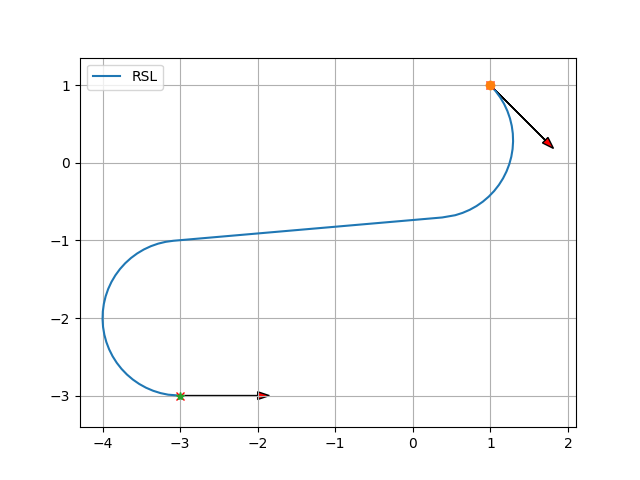
\includegraphics[width=0.8\textwidth]{fig/dubins/dubins_example.png}
\caption{Dubins path starting from point (1, 1) with heading angle $\frac{-\pi}{4}$ and ending at (-3, -3) with heading angle 0}
\label{fig:dubins_example}
\end{figure}

\subsection{CSC Dubins Path}

The CSC trajectories include RSR, LSR, RSL, and LSR, which stands for a turn followed by a straight line followed by another turn (Shown in Figure \ref{fig:dubins pattern CSC}).

Pick a position and orientation for your start and goal configurations. Draw your start and goal configurations as points in the plane with arrows extending out in the direction the car is facing. Next, draw circles to the left and right of the car with radius $r_{min}$ . The circles should be tangent at the location of the car. Draw tangent lines from the circles at the starting configuration to the circles at the goal configuration. In the next section I’ll discuss how to compute this, but for now just draw them.

For every pair of circles, whether it's RR, LL, RL, or LR, four potential tangent lines can be drawn. However, only one of these lines for each pair is valid. Specifically, for the RR circles, a single line drawn from the agent's circle intersects the goal's circle in a manner that ensures the correct direction, whose Dubins trajectory can be simplified as RR without S in between. As a result, for any CSC Trajectory, there exists a distinct tangent line to be followed. This line represents the 'S' segment of the trajectory. The points where this line touches the circles are the critical points the agent needs to navigate through to complete its path. Essentially, determining these trajectories hinges on accurately identifying these tangent points.

\begin{figure}
     \centering
     \begin{subfigure}[b]{0.2\textwidth}
         \centering
         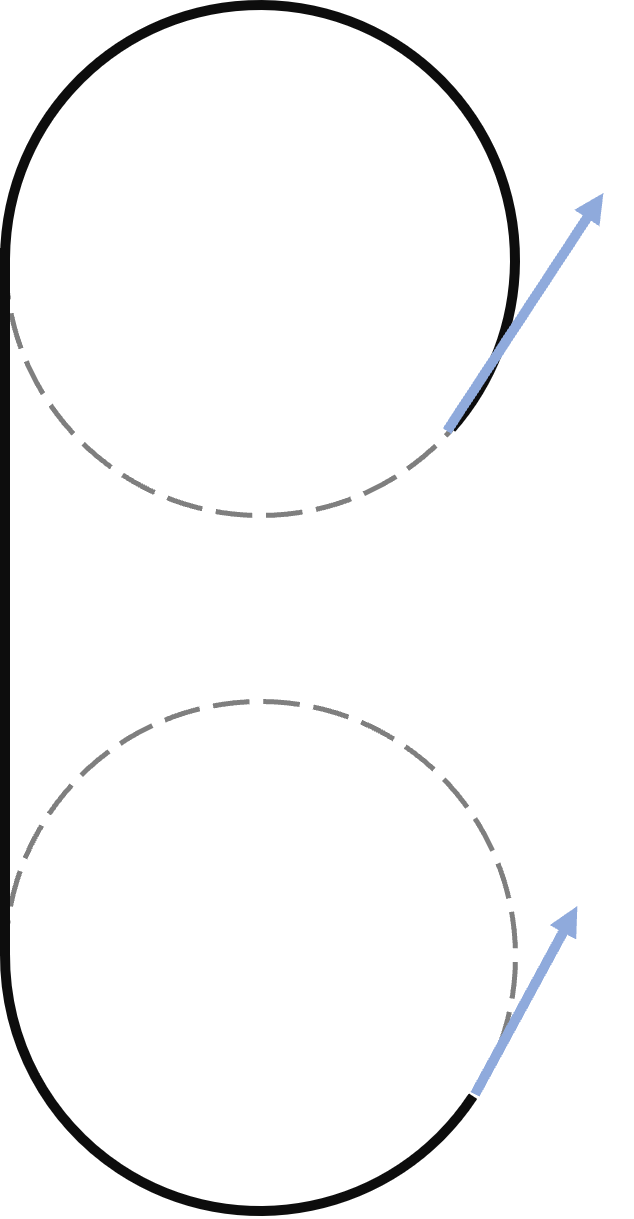
\includegraphics[scale=0.7]{fig/dubins/LSL.png}
         \caption{dubins pattern LSL}
         \label{fig: dubins pattern LSL}
     \end{subfigure}
     \hfill
     \begin{subfigure}[b]{0.2\textwidth}
         \centering
         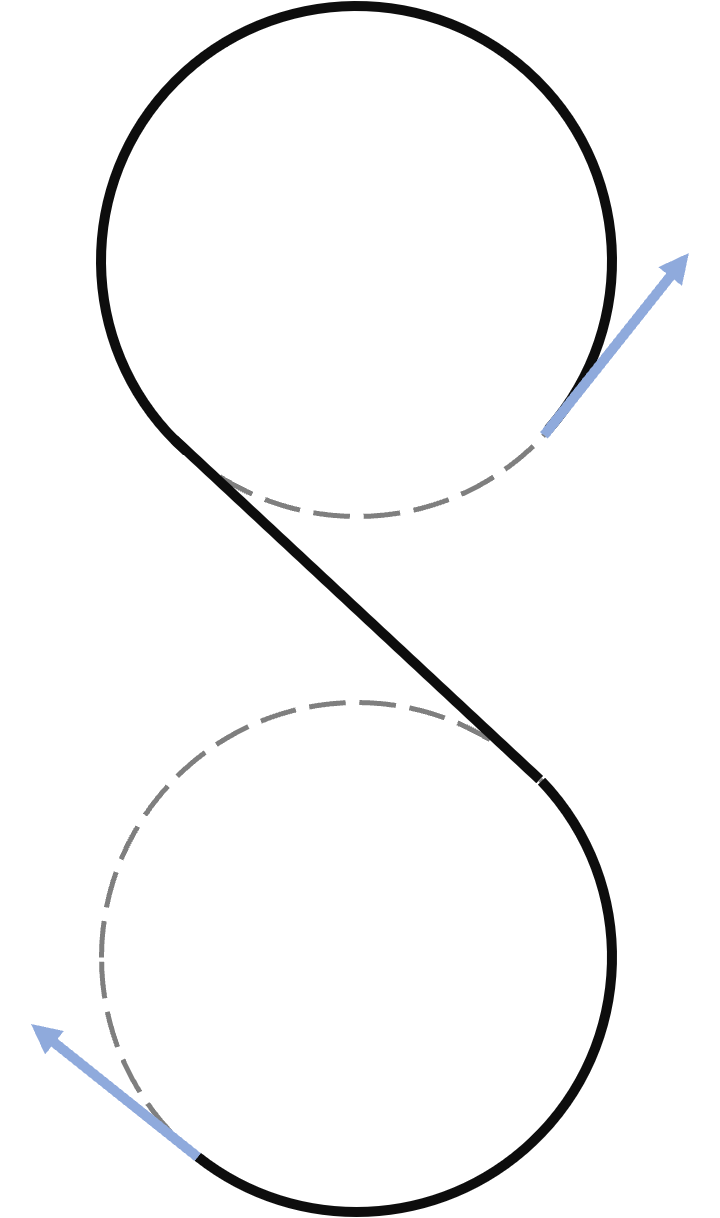
\includegraphics[scale=0.7]{fig/dubins/LSR.png}
         \caption{dubins pattern LSR}
         \label{fig:dubins pattern LSR}
     \end{subfigure}
     \hfill
     \begin{subfigure}[b]{0.2\textwidth}
         \centering
         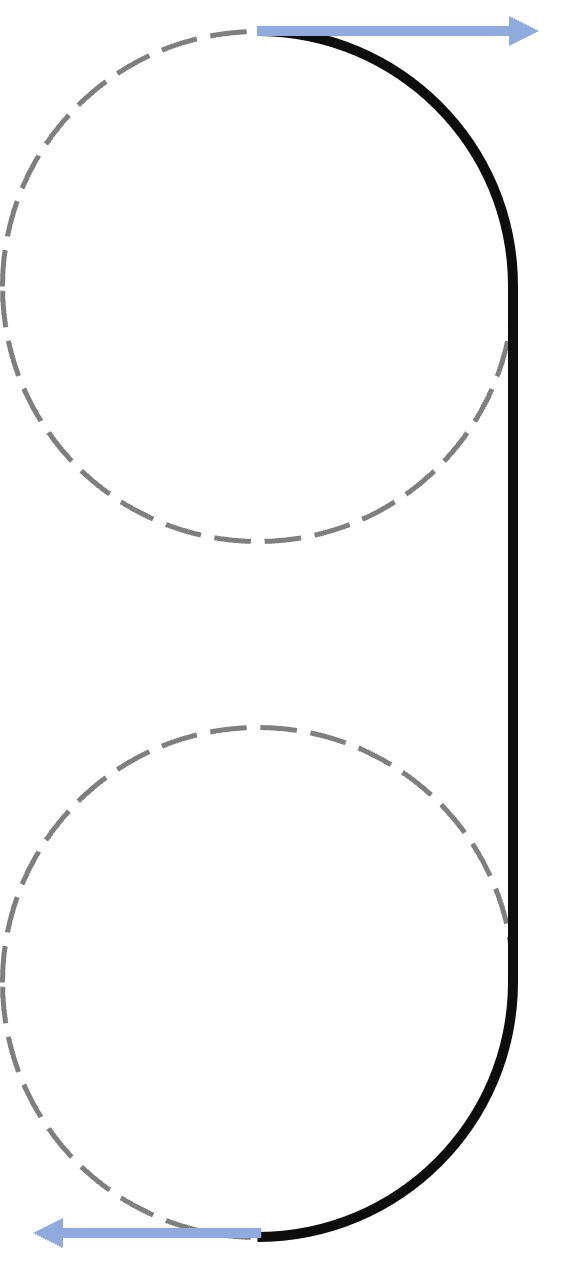
\includegraphics[scale=0.7]{fig/dubins/RSR.png}
         \caption{dubins pattern RSR}
         \label{fig:dubins pattern RSR}
     \end{subfigure}
     \hfill
     \begin{subfigure}[b]{0.2\textwidth}
         \centering
         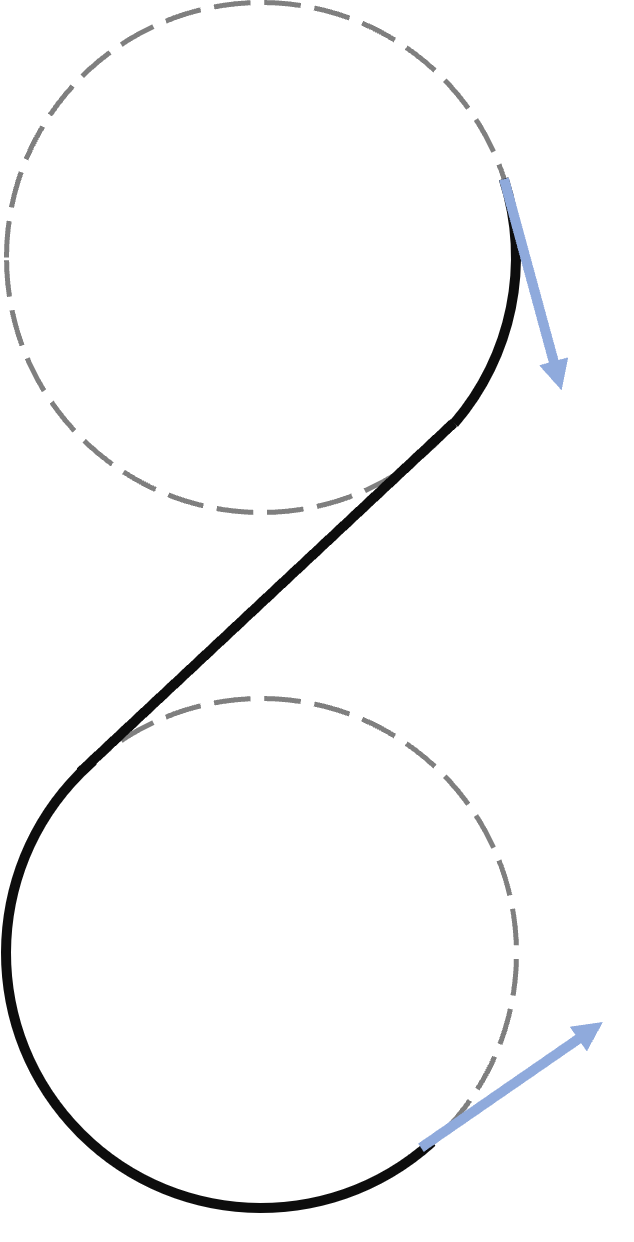
\includegraphics[scale=0.7]{fig/dubins/RSL.png}
         \caption{dubins pattern RSL}
         \label{fig:dubins pattern RSL}
     \end{subfigure}
        \caption{Four patterns under CSC type }
        \label{fig:dubins pattern CSC}
\end{figure}

\subsection{CCC Dubins path}

The CCC trajectories is different from CSC in the connection path, which only involve an initial turn, followed by a turn in the opposite direction, and then revert to the initial turning direction, as exemplified by the RLR Trajectory in Figure \ref{fig:dubins pattern CCC}. These trajectories are applicable when the ego vehicle and the target position are close within a threshold. If they aren't, one of the circles would necessitate a radius exceeding $r_{min}$ . In such cases, the CCC Trajectory becomes less than ideal. For the Dubin's path planning, there are only two types of CCC trajectories: RLR and LRL. Simply determining the tangent lines between RR or LL circles isn't sufficient in this context. The third circle between the starting and finishing circle in the trajectory remains tangent to both the starting and finishing turning circles. However, the points of tangent differ from those derived from standard tangent line computations. 

\begin{figure}
     \centering
     \begin{subfigure}[b]{0.4\textwidth}
         \centering
         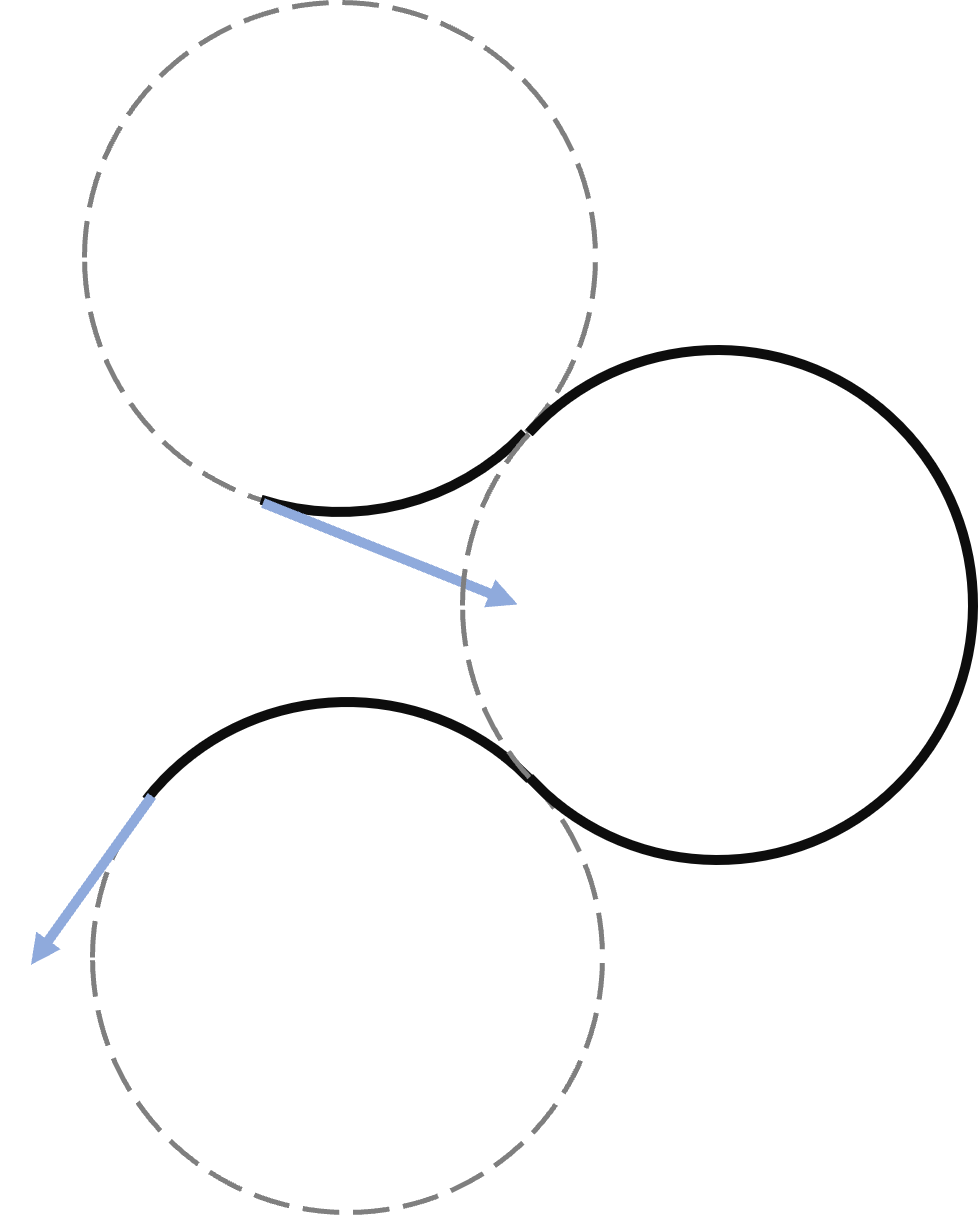
\includegraphics[scale=0.7]{fig/dubins/LRL.png}
         \caption{dubins pattern LRL}
         \label{fig: dubins pattern LRL}
     \end{subfigure}
     \hfill
     \begin{subfigure}[b]{0.4\textwidth}
         \centering
         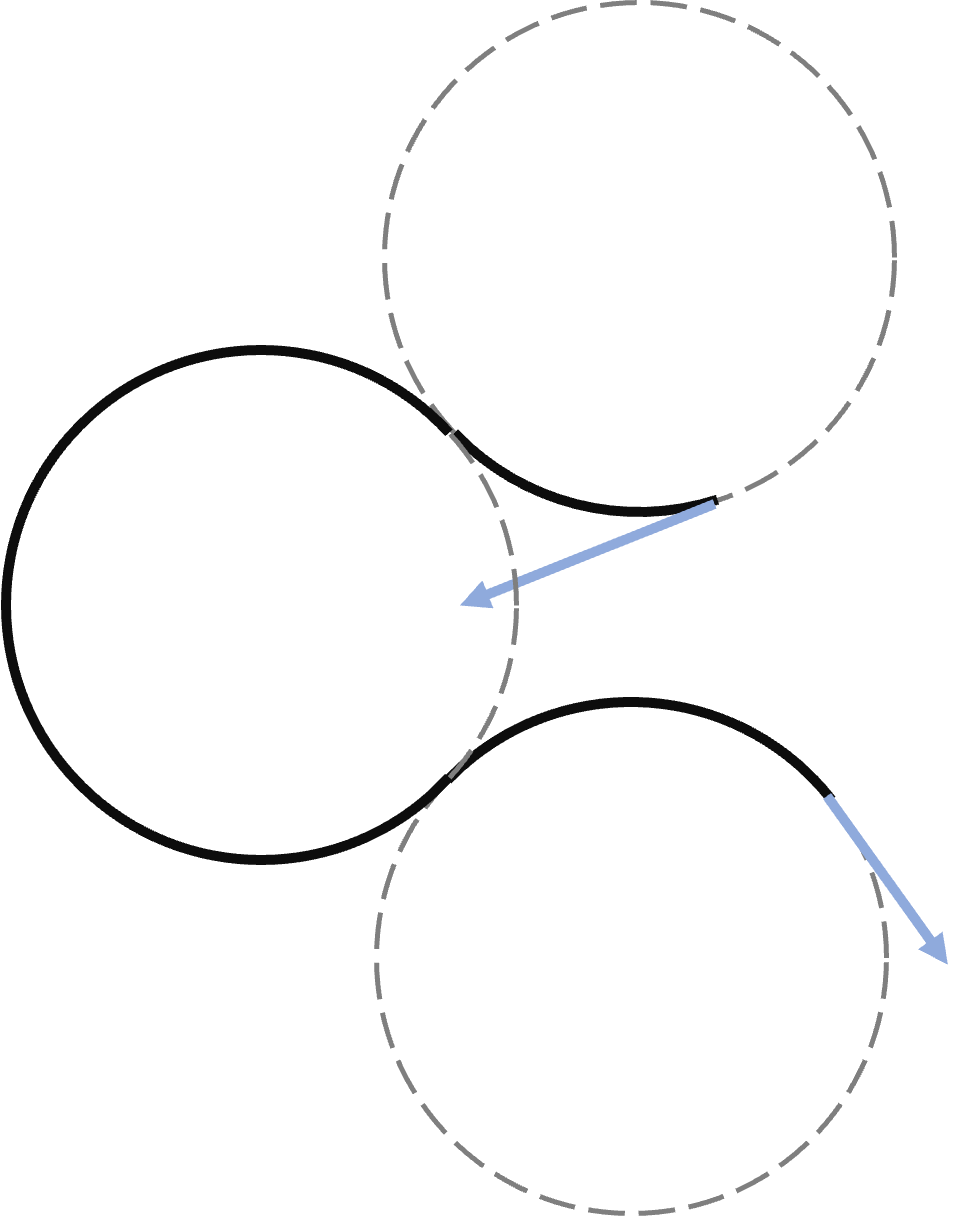
\includegraphics[scale=0.7]{fig/dubins/RLR.png}
         \caption{dubins pattern RLR}
         \label{fig:dubins pattern RLR}
     \end{subfigure}
        \caption{Four patterns under CCC type }
        \label{fig:dubins pattern CCC}
\end{figure}


\subsection{Construction of Dubins path}

Consider the following input parameters.
\begin{enumerate}
\item Initial pose of the target: $P_s\left(x_s, y_s, \theta_s\right)$
\item Final pose of the target: $P_f\left(x_f, y_f, \theta_f\right)$
\item Initial turning radius: $\rho_s\left(=\frac{1}{\kappa_s}\right)$
\item Final turning radius: $\rho_f\left(=\frac{1}{\kappa_f}\right)$
\end{enumerate}
where the initial turning radisu and final turning radius is equal for vehicle path planning, which is determined by vehicle steering angle:
\begin{equation}
    R = \frac{L}{tan(\delta)}
\label{eq: turning radius using delta}
\end{equation}

To compute the Dubins path, we need to start from the two turning circle center $O_s\left(x_{c s}, y_{c s}\right)$ and $O_f\left(x_{c f}, y_{c f}\right)$, which can be computed as:
\begin{align}
    &\left(x_{c s}, y_{c s}\right)=\\ \notag
        &(x_s \pm \rho_s \cos \left(\theta_s \pm \frac{\pi}{2}\right), y_s \pm \rho_s \sin \left(\theta_s \pm \frac{\pi}{2}\right)) 
\end{align}
\begin{align}
        &\left(x_{c f}, y_{c f}\right)=\\ \notag
        &(x_f \pm \rho_f \cos \left(\theta_f \pm \frac{\pi}{2}\right), y_f \pm \rho_f \sin \left(\theta_f \pm \frac{\pi}{2}\right))
\end{align}

Then, the reference circle of radius $\left|\rho_f-\rho_s\right|$ is constructed at $O_f$ for $\rho_s \leq \rho_f$, and the two primary circle center is connected with center reference line:
\begin{equation}
    |c|=\sqrt{\left(x_{c s}-x_{c f}\right)^2+\left(y_{c s}-y_{c f}\right)^2}
\end{equation}

A perpendicular line to $c$ at $O_f$ intersects the reference circle at a point $T^{\prime}$ and the primary circle $C_f$ at the tangent entry point $T_{ent}$. A line from $O_s$ to $T^{\prime}$ is drawn, and another line parallel to $O_f T_{ent}$ is extended from $O_s$ to meet $C_s$ at the tangent exit point $T_{ext}$. The path is completed by connecting the starting position $P_s$ to $T_{ext}$ with an arc of radius $\rho_s$, and from $T_{ent}$ to the finishing position $P_f$ with an arc of radius $\rho_f$. The resulting composite path consists of the starting arc $P_s T_{ext}$, the external tangent line $T_{ext} T_{ent}$, and the ending arc $T_{ent} P_f$. To determine the shortest Dubins path between the same initial and final points, multiple patterns are considered in Figure \ref{fig:dubins pattern difference for same condition}, and the one with the least total length is selected.

\begin{figure}
     \centering
     \begin{subfigure}[b]{0.8\textwidth}
         \centering
         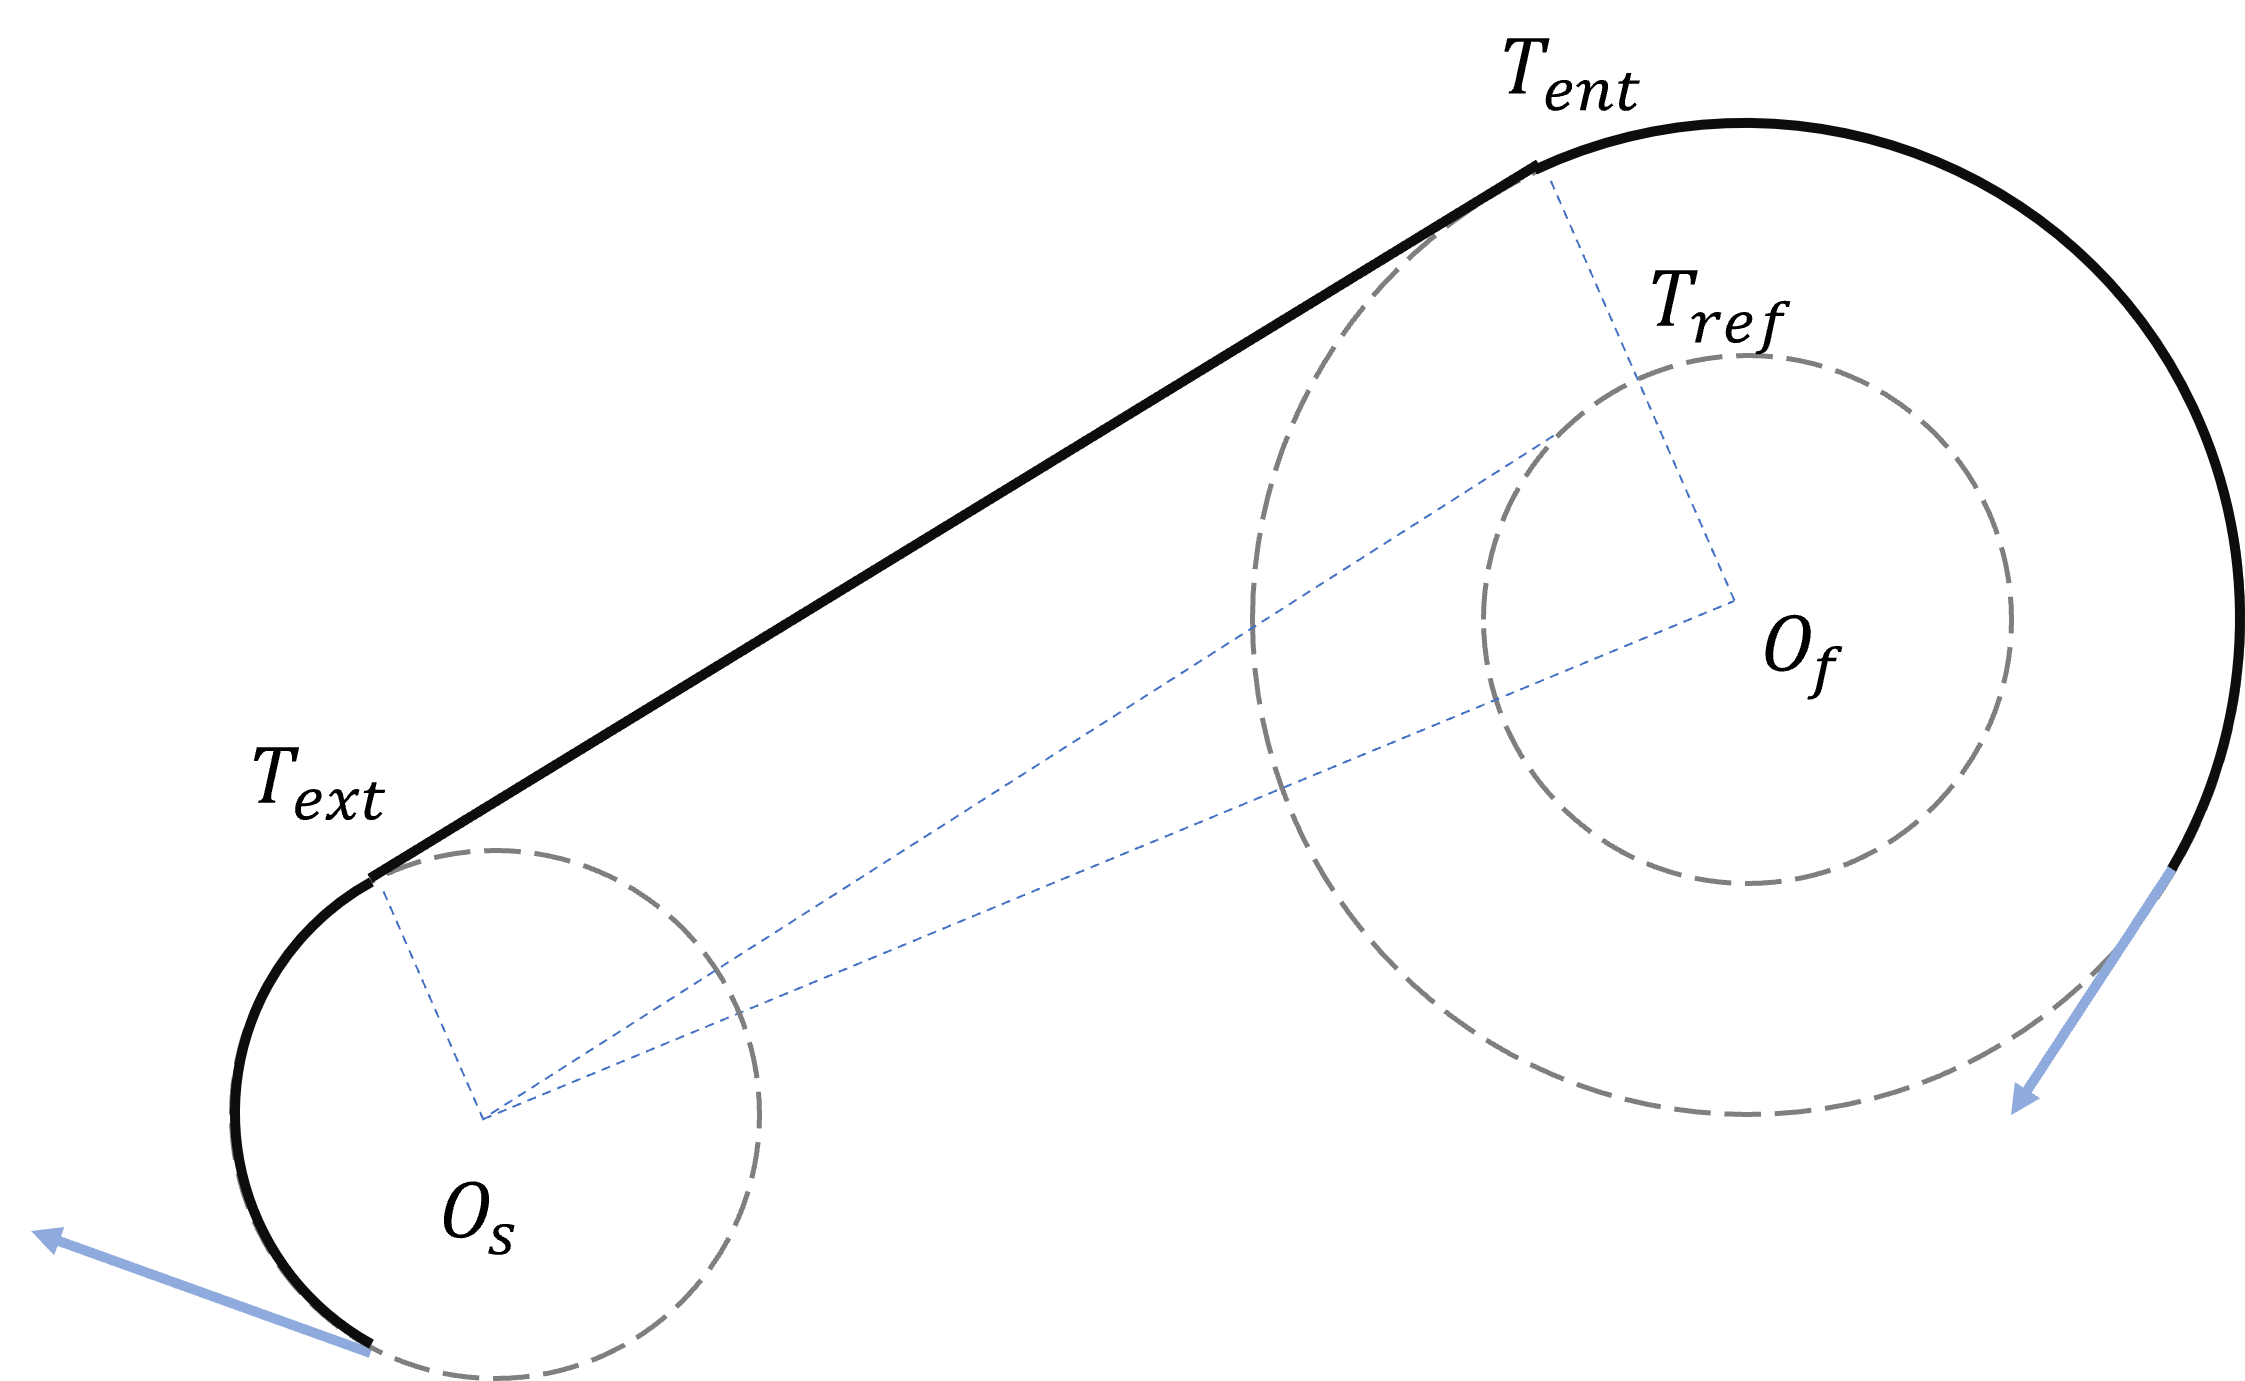
\includegraphics[width=0.7\linewidth]{fig/dubins/dubins_construction_rsr.png}
         \caption{Dubins construction following RSR pattern}
         \label{fig: dubins pattern consturction RSR}
     \end{subfigure}
     \vfill 
     \begin{subfigure}[b]{0.8\textwidth}
         \centering
         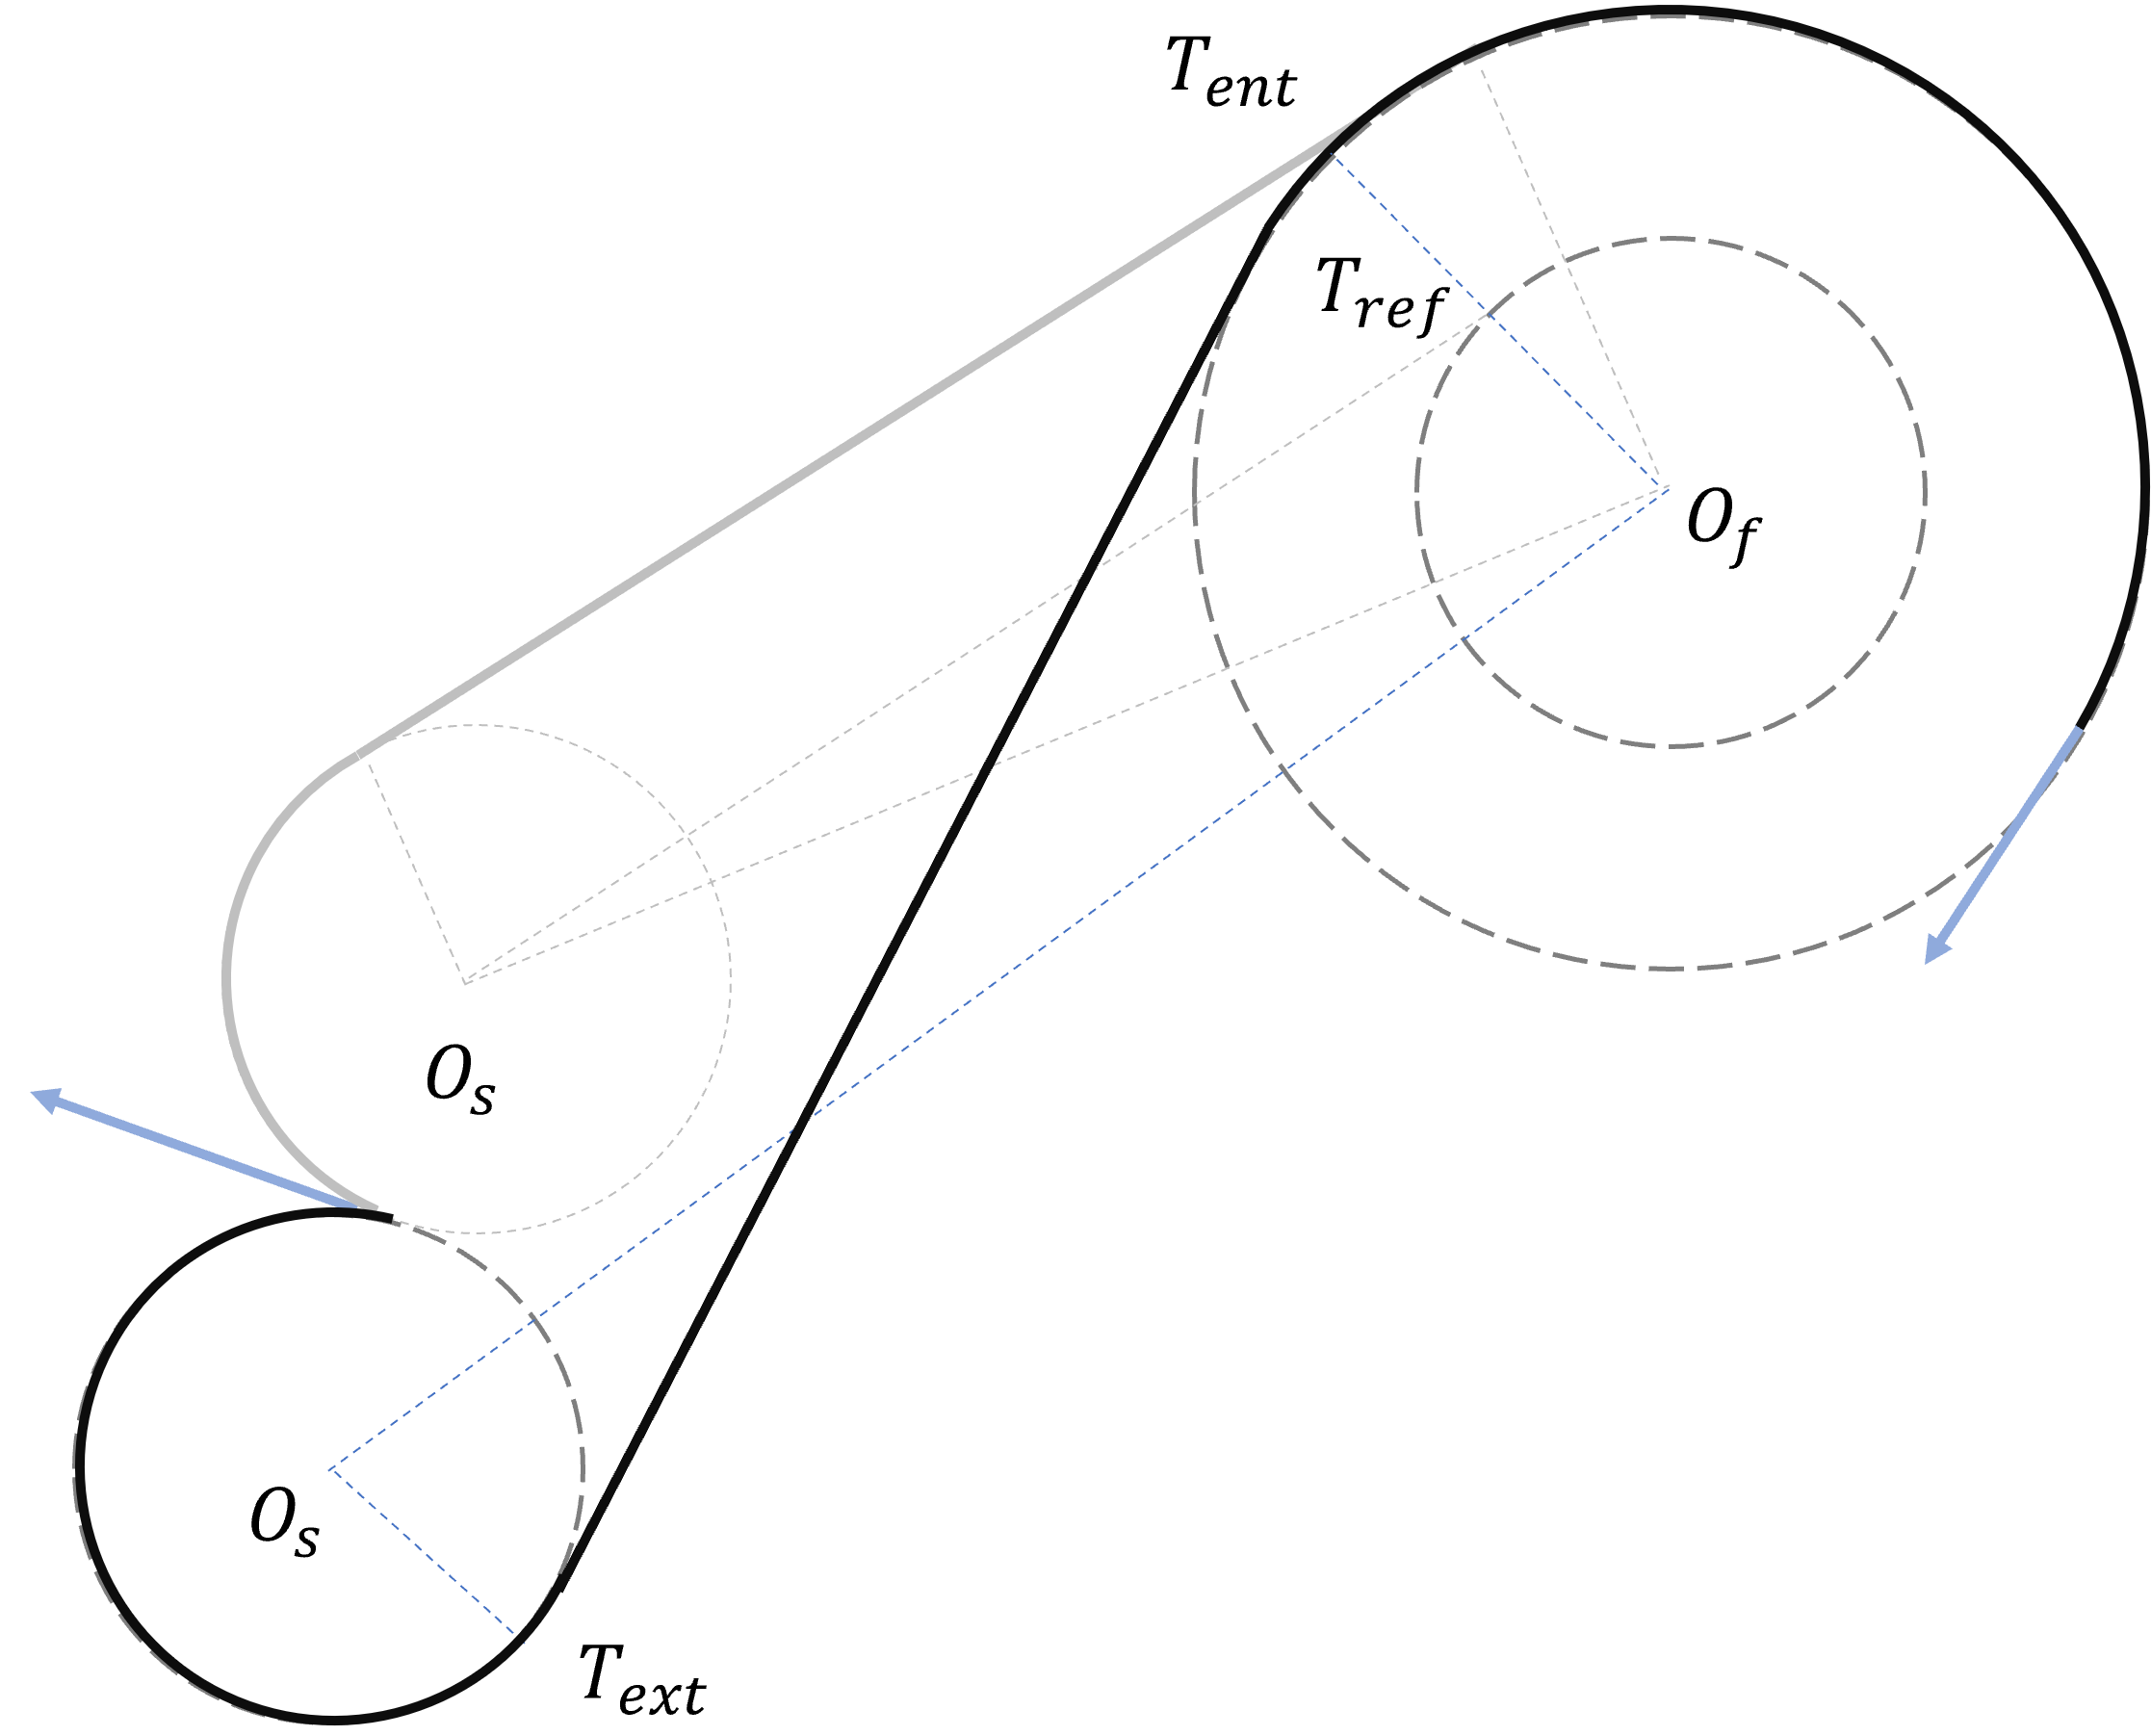
\includegraphics[width=0.7\linewidth]{fig/dubins/dubins_construction_lsr.png}
         \caption{Dubins construction following LSR pattern, the pattern for RSR is in grey color for comparison}
         \label{fig: dubins pattern consturction LSR}
     \end{subfigure}
        \caption{Different Dubins contruction pattern for the same start and finish condition}
        \label{fig:dubins pattern difference for same condition}
\end{figure}

\section{LQR controller design for TTWR}

The first control algorithm implemented in the traditional hierarchy TTWR controller is the Linear Quadratic Regulator (LQR). As defined in Section \ref{section: ttwr system analysis}, the system $(\mathcal{A}, \mathcal{B})$ is controllable by analysing its controllaiblity grammian or by applying Cayley-Hamilton theorem to its controllability matrix, which indicates that it is possible to manipulate the eigen values of the closes loop system $(\mathcal{A} - \mathcal{B}K)$ by choosing the state feed back control law $u = -K x$. Similarly, the LQR algorithm is a widely used algorithm to find an appropriate state-feedback controller. LQR controllers possess inherent robustness with guaranteed gain and phase margin \parencite{lehtomaki1981robustness}, and LQR plays a crucial role in addressing the LQG (linear–quadratic–Gaussian) challenge, which is the foundational problems in control theory.

For a controllable system, given either full-state measurements or full-state estimate, there exists more than one control laws, $u = - K x$, which stabilize the system states, and the eigenvalues of the closed-loop system, $(A - B K)$, can be designed and placed to left-half of the complex plane to achieve system stability. However, over stability by choosing large negative eigenvalues might require significant large control efforts, and may exceed the system input limitation, cause a wast of control energy, and reduce the system robustness for certain noise and disturbance. Therefore, the balance between stability of the closed loop system and the aggressiveness of the control input is the main purpose in optimal control, which is achieved by choosing the most suitable gain matrix K to stabilize the system without expending too much control effort. Three rules shall be taken into consideration when choosing the proper control gain, which incluldes \parencite{brunton2022data}:

\begin{itemize}
    \item prevent the controller from overreacting to high-frequency noise and disturbances
    \item the control actuation does not exceed limitation
    \item the control effort is not prohibitively expensive
\end{itemize}

For an infinite-horizon, continuous-time system described in Equation \ref{eqn: lti system states}, the cost function defined as:
\begin{equation}
    J=\int_0^{\infty}\left(x^T Q x+u^T R u+2 x^T N u\right) d t
    \label{eqn: lqr control cost function}
\end{equation}
where the matrices $Q$ and $R$ weight the cost of state deviation and actuation cost respectively, the matrix $Q$ is positive semi-definite, and $R$ is positive definite; these matrices are often diagonal, and the diagonal elements can be tuned to change the relative importance of the control objectives.

\begin{figure}
    \centering
    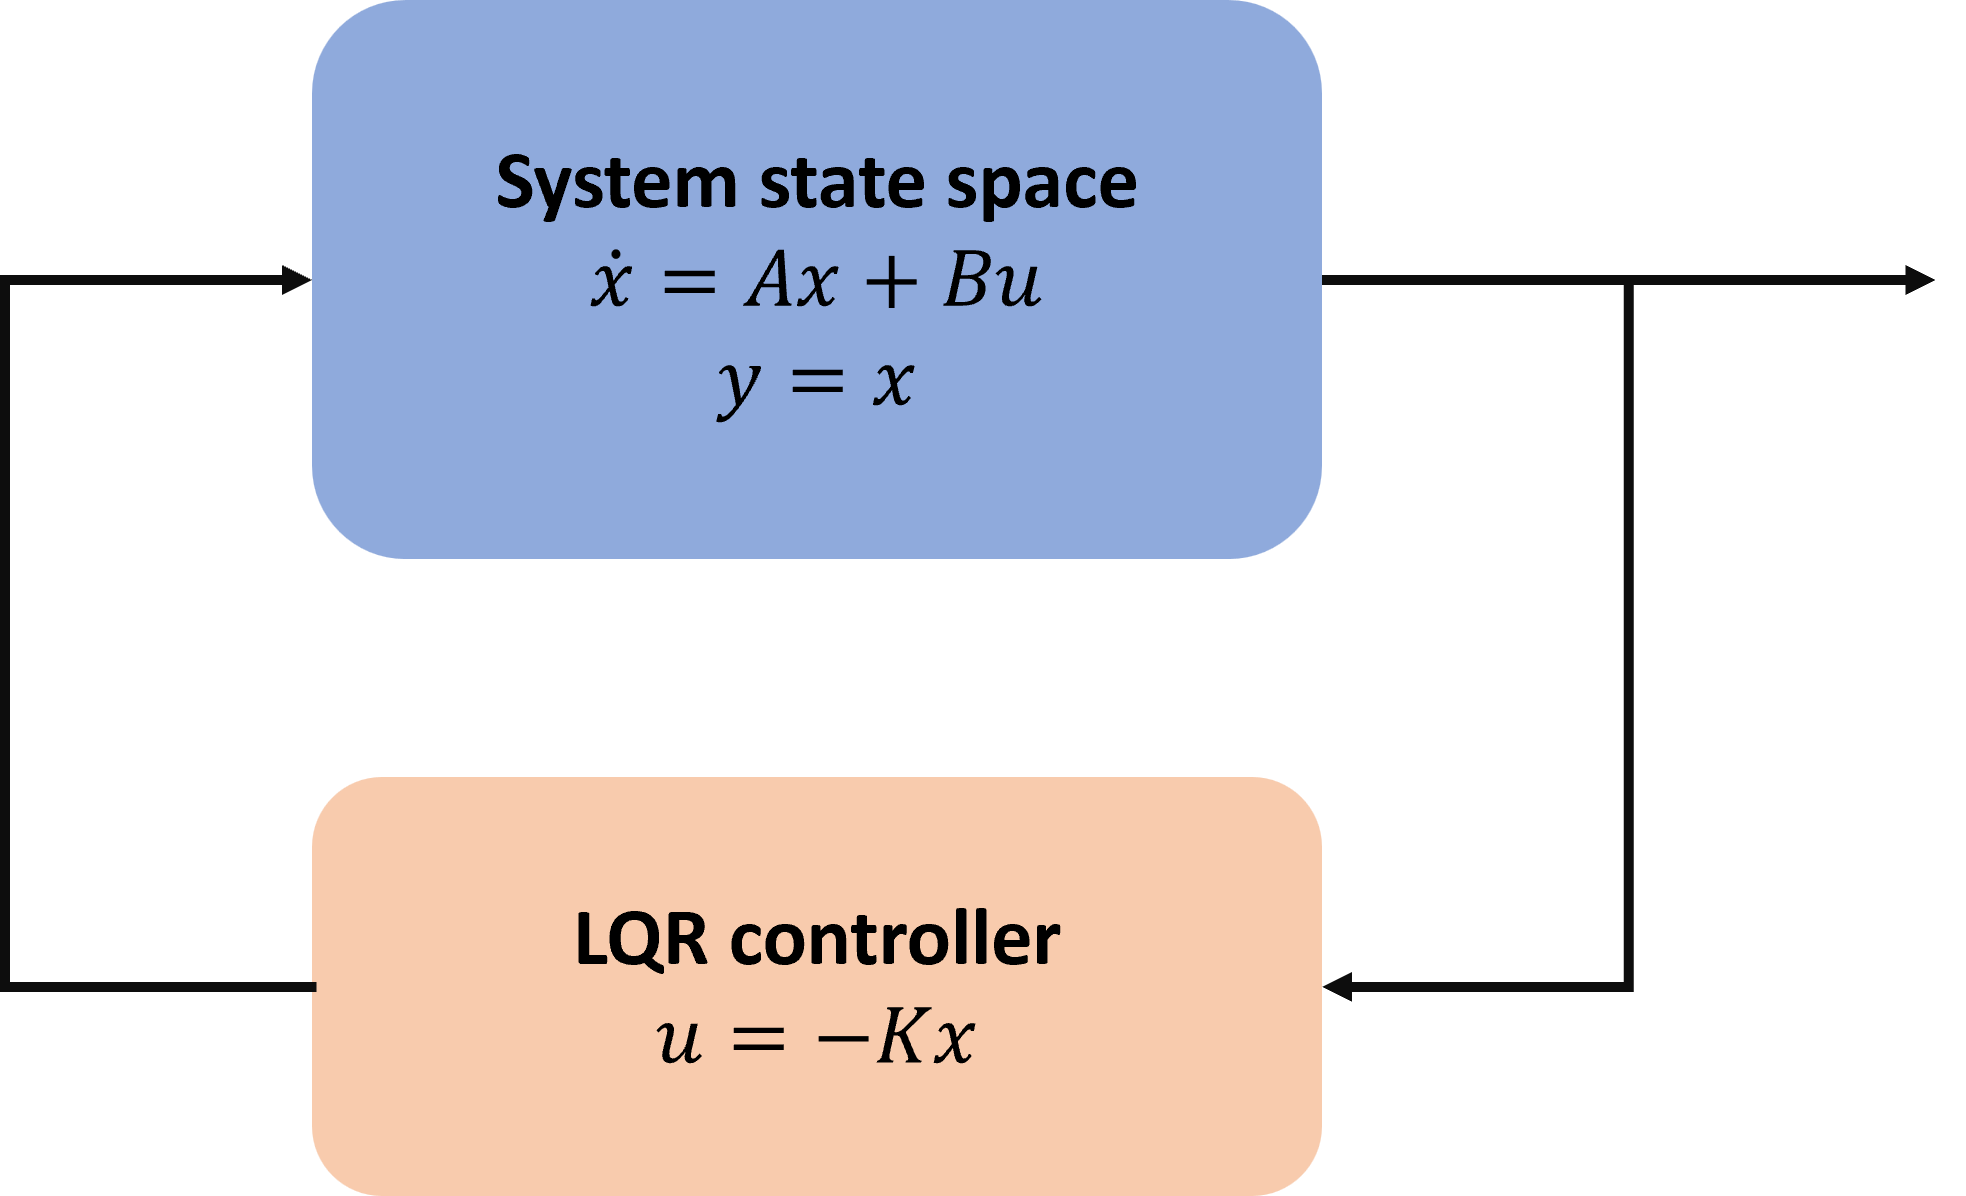
\includegraphics[width=0.5\linewidth]{fig/lqr_control_example.png}
    \caption{LQR controller schematic diagram}
    \label{fig: LQR controller schematic diagram}
\end{figure}

The weight matrix is useful to make choices to optimize the control law, for example, a larger value in a particular diagonal entry of $Q$ matrix means that deviations in the corresponding state will be penalized more heavily in the cost function. This will lead the controller to work harder to regulate the particular state. When the $Q$ matrix is set to be zero, the controller will not attempt to regulate the state at all, focusing solely on minimizing control effort. The matrix $R$ determines how much the control actions are penalized in the cost function. A larger value in a diagonal entry of R means that the corresponding control action will be penalized more. This discourages aggressive control actions and can be used to ensure smoother control signals. If R is too small, the controller might become overly aggressive, leading to large control signals that could saturate actuators or cause wear and tear.

As shown in Figure \ref{fig: LQR controller schematic diagram}, the LQR control law $u = - K x$ is designed to minimize the cost function $J=\lim _{t \rightarrow \infty} J(t)$. As its name suggests, LQR is a control strategy formulated for linear systems and employs the linear control law to minimize a cost function defined quadratically, aims to optimally regulate the system's state $\lim _{t \rightarrow \infty} \mathbf{x}(t)=0$. The analytical solution for the optimal controller gain $K$ can be computed following:
\begin{equation}
    K=R^{-1}\left(B^T P+N^T\right)
\end{equation}
and the variable $P$ is found by solving the continuous time algebraic Riccati equation:
\begin{equation}
    A^T P+P A-(P B+N) R^{-1}\left(B^T P+N^T\right)+Q=0
\end{equation}
which can be also written as:
\begin{equation}
    \mathcal{A}^T P+P \mathcal{A}-P B R^{-1} B^T P+\mathcal{Q}=0
\end{equation}
with
\begin{equation}
    \mathcal{A}=A-B R^{-1} N^T \quad \mathcal{Q}=Q-N R^{-1} N^T
\end{equation}

\begin{figure}
    \centering
    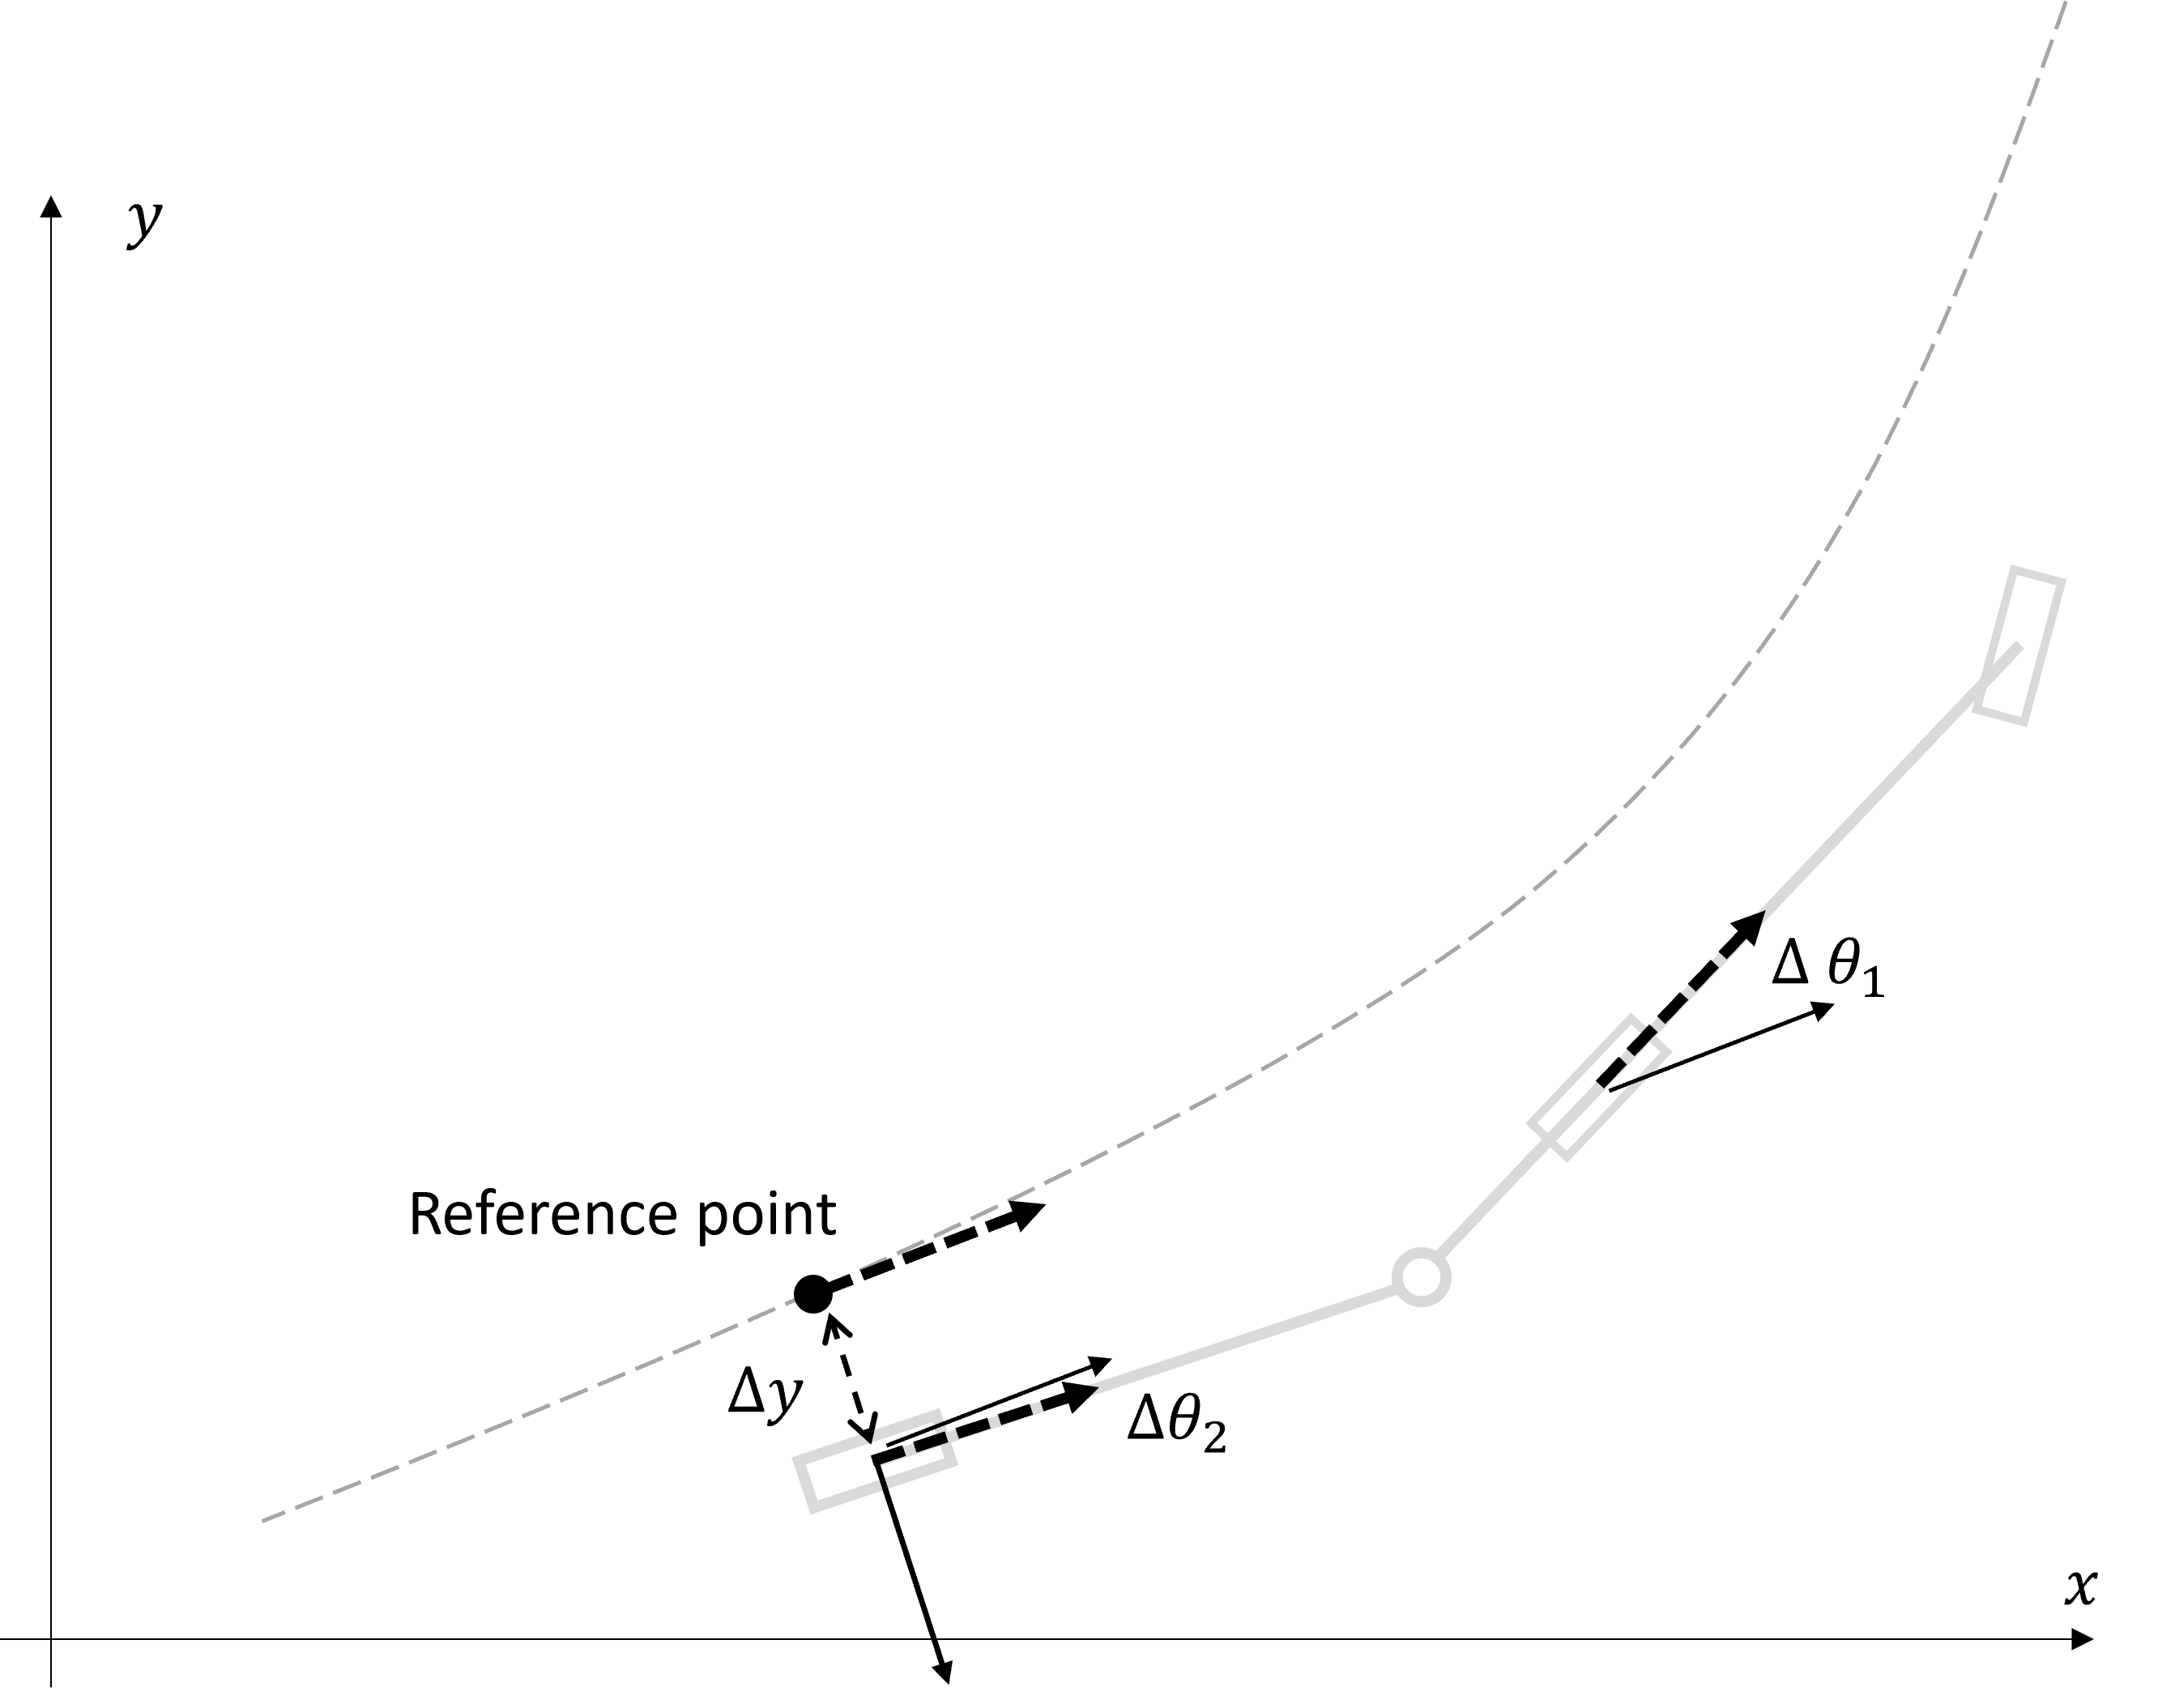
\includegraphics[width=0.7\linewidth]{fig/lateral distance error.png}
    \caption{LQR controller reference states error}
    \label{fig: LQR controller reference states error}
\end{figure}

For the TTWR control topic, the state equation can be formulated as:
\begin{equation} 
\begin{bmatrix}
    \Delta \dot{\theta_1} \\ \Delta \dot{\theta_2} \\ \Delta \dot{y}
\end{bmatrix} = \begin{bmatrix}
0 & 0 & 0 \\
\frac{v}{L_3} & -\frac{v}{L_3} & 0 \\
0 & V & 0
\end{bmatrix}   \begin{bmatrix}
    \Delta \theta_1 \\ \Delta \theta_2 \\ \Delta y
\end{bmatrix} + \begin{bmatrix}
    \frac{v}{L_1} \\ -\frac{L_2}{L_1  L_3} v \\ 0
\end{bmatrix} \delta \label{eq: lqr state space}\end{equation}
as shown in Figure \ref{fig: LQR controller reference states error}, the reference states error consist of $\Delta \theta_1$, $\Delta \theta_2$, and $\Delta y$, which represents the heading error between TTWR's truck heading angle and the reference point heading angle, the heading error between trailer heading angle and reference point heading angle, and the lateral distance in trailer coordinate between trailer position and refernece point.

To compute the optimal gain of the TTWR controller, MATLAB provides built-in functions which can solve Riccati equation efficiently by providing the system state space model, weight matrix $Q$ and $R$, the code is as following:

\begin{lstlisting}[
frame=single,
numbers=left,
style=Matlab-Pyglike]
% TTWR parameters
L1 = 3; % truck wheelbase length [m]
L2 = 2; % hitch length [m] 
L3 = 1.5; % trailer wheelbase length [m] 
vx = -2; % truck longitudinal velocity [m/s] 

% Linearized State Space
A = [0       0         0;
     vx./L3  -vx./L3   0;
     0       vx        0];

B = [vx./L1;
     -L2*vx ./ (L1*L3);
     0];

C = eye(3);
D = zeros(3, 1);

% state states x = [\theta1, \theta2, \y_err]
sys = ss(A, B, C, D);

% State weight matrix
% \theta1 and \theta2 error ref for 2 degrees, and  
% lateral error reference value is 0.8
Q = [1/(deg2rad(2).^2)       0                       0;
     0                   1/(deg2rad(2).^2)           0;
     0                        0                1/(0.8.^2)];
% Input weight matrix for steering angle
R = 1 / (deg2rad(steer_max).^2);

% Output K is the LQR gain
[K,S,P] = lqr(sys, Q, R)
\end{lstlisting}

\begin{figure}
    \centering
    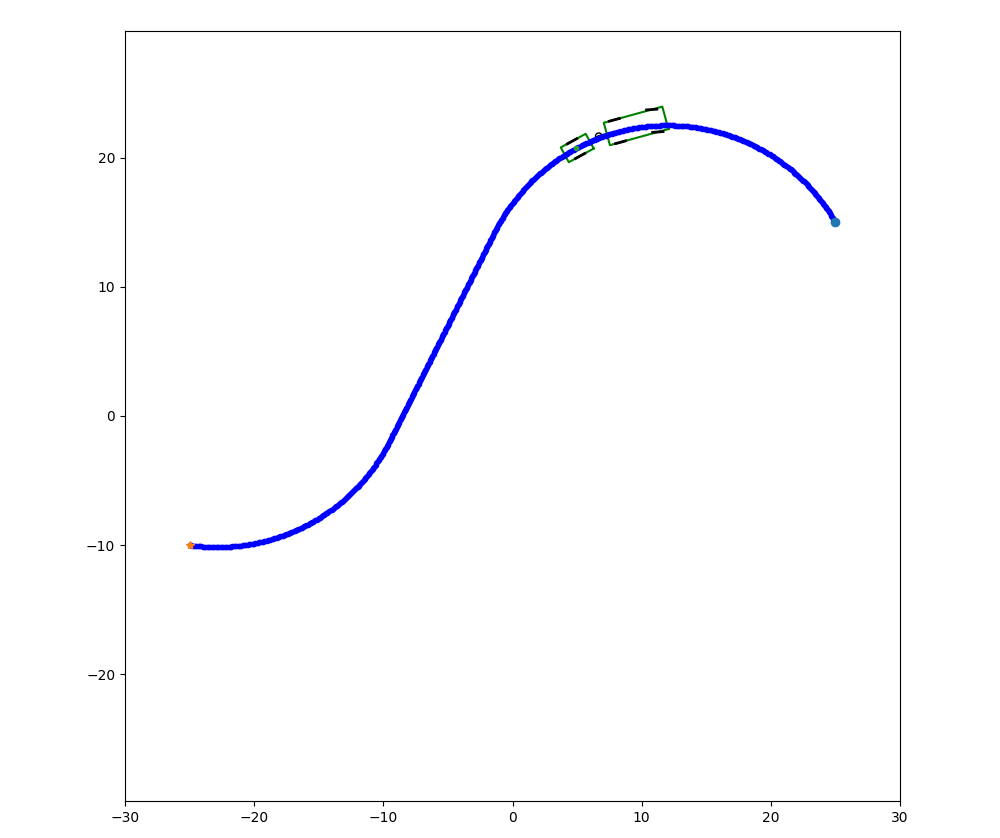
\includegraphics[width=0.8\linewidth]{fig/lqr/lqr_path_following.png}
    \caption{The simulation of using Dubins and LQR for TTWR reverse driving control}
    \label{fig: simulation of using Dubins and LQR for TTWR reverse driving control}
\end{figure}

\begin{figure}
    \centering
    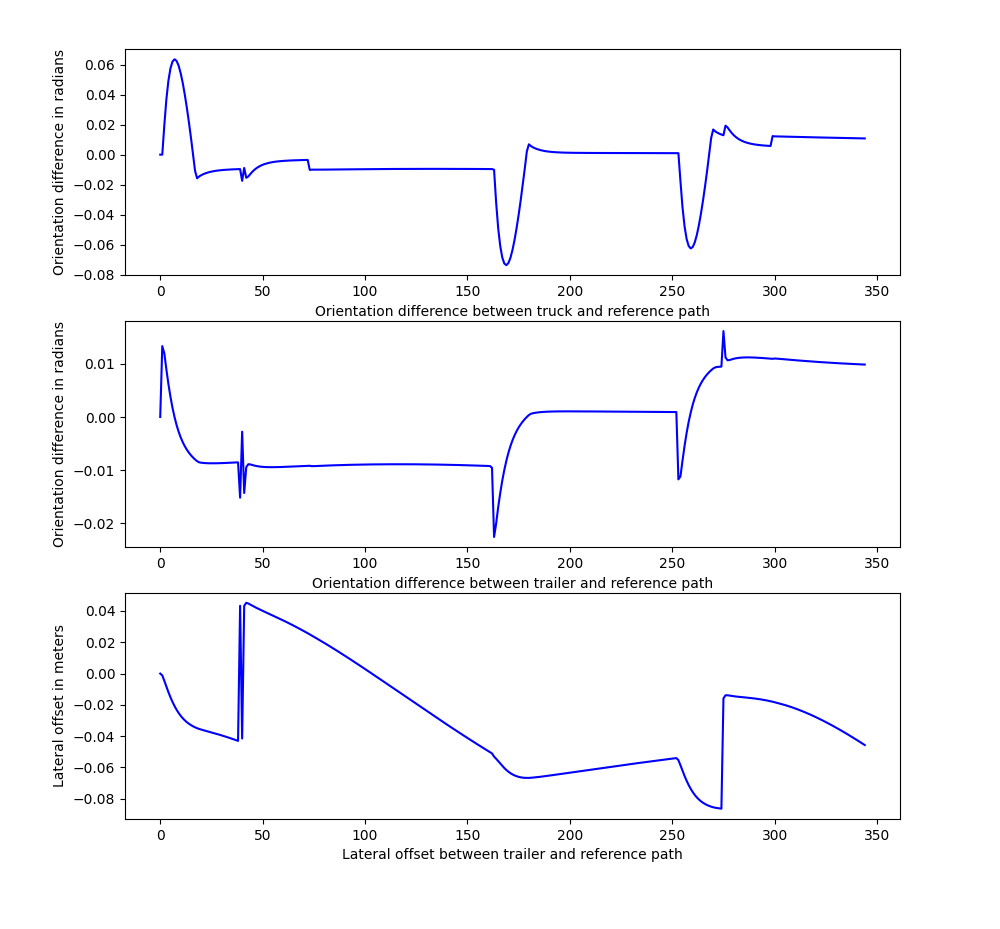
\includegraphics[width=0.7\linewidth]{fig/lqr/lqr states.png}
    \caption{The system states of the LQR controller}
    \label{fig: system states of the LQR controller}
\end{figure}

The results of the LQR TTWR reverse path following control is shown in Figures \ref{fig: simulation of using Dubins and LQR for TTWR reverse driving control}, which depict the reference trajectory and the TTWR vehicle states respectively. The blue line is the Dubins trajectory started with initial states $(25, 25, -\frac{\pi}{3})$ and final states $(-25. -10, 0)$ which is lateral offset between trajectory and truck or trailer, and the heading angle difference between trajectory and trailer. The Figure \ref{fig: system states of the LQR controller} shows the TTWR states along the path following task, and the lateral offset of truck and traler are both within 0.1 meters, and the heading angle difference is also within 0.1 rad. The LQR controller effectively ensures that the articulated vehicle system follows closely to the desired trajectory. This is evident from the gentle turning motions observed whenever the blue line alters its direction. Moreover, the consistent spacing between each sample signifies a gradual and smooth turning process, highlighting the controller's efficiency in maintaining steady and controlled maneuvers.

\clearpage

\section{MPC controller design for TTWR}
\label{MPC controller design for TTWR}
Model Predictive Control (MPC) operates by executing finite-horizon optimization for a system model at each discrete time step. The primary idea behind MPC is to use a model of the system to predict its future behavior over a finite horizon. Based on this prediction, the control inputs are determined by minimizing a cost function, which typically represents a combination of tracking errors and control efforts.
\begin{equation}
J = \sum_{k=0}^{N-1} \left( x(k)^T Q x(k) + u(k)^T R u(k) \right) + x(N)^T P x(N)
\end{equation}
where $J$ is the cost to be minimized, $N$ is the prediction horizon, $X_k$ is the system states at time $t_k$, $U_k$ is the input states at time $t_k$, and $Q$ and $R$ is the weight matrix for system states and control input respectively, and these two matrices are designed to be positive definite, and the $P$ is the terminal cost wight matrix.

At every instance $t_k$, the system is sampled, and a control strategy is derived for the control horizon $[t_k, t_k + N_C]$ to minimize the deviation from the desired trajectory over the prediction horizon $[t_k, t_k + N_P]$. Beyond $N_C$ control moves, the control input remains constant for the rest of the prediction horizon. The system's progression is forecasted using an intrinsic mathematical model, and a numerical optimization technique minimizes the control cost. Only the initial control input from the determined sequence is implemented at each time step $t_k$. This procedure is repeated in every cycle, with both the control and prediction horizons advancing forward. The principle of the MPC algorithm is shown in Figure \ref{fig: Function principle of a model-based predictive}.

\begin{figure}
    \centering
    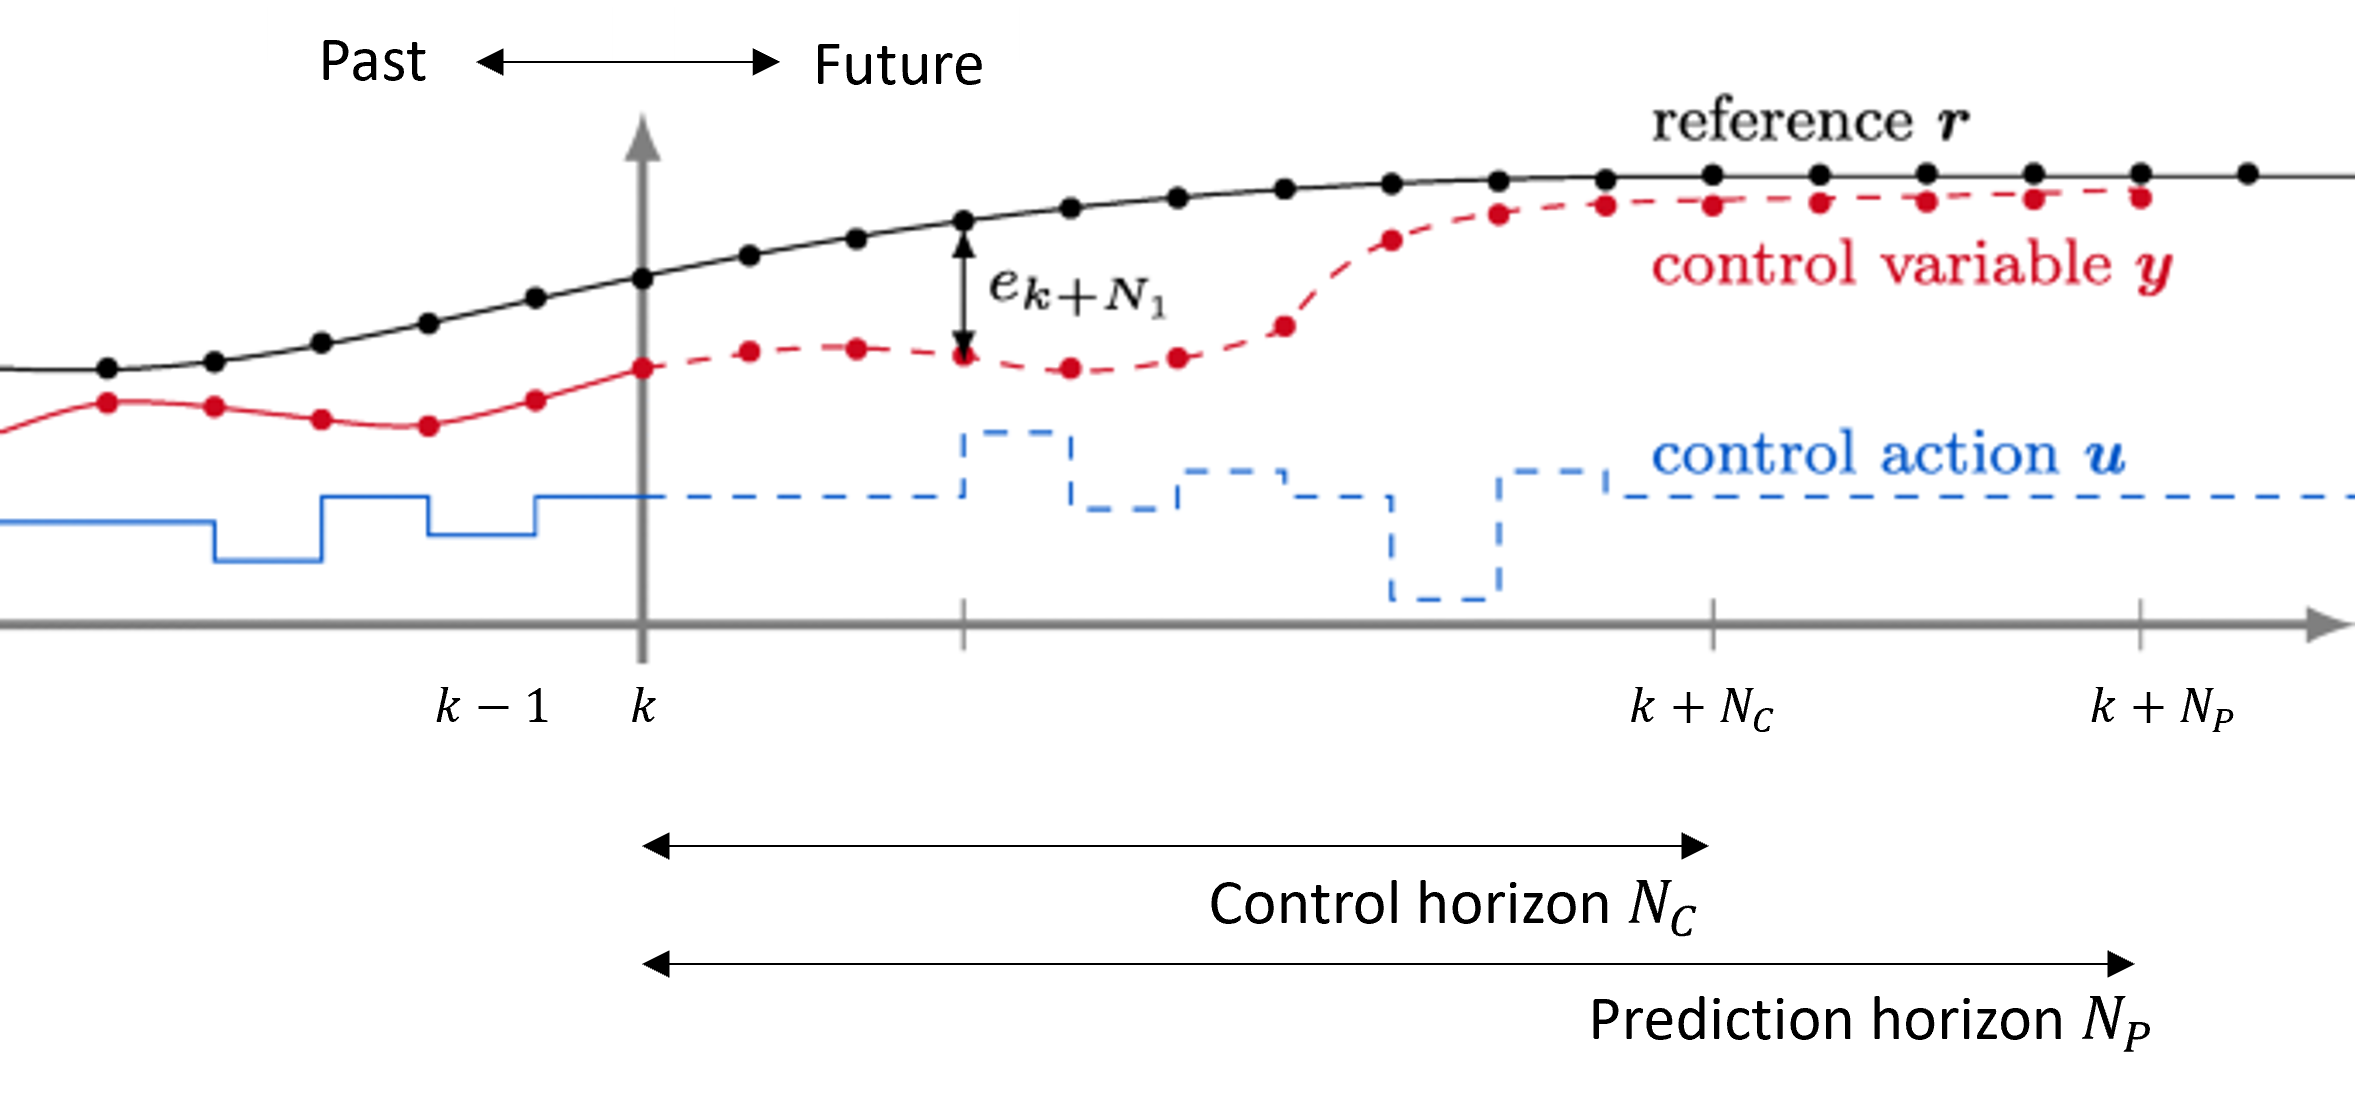
\includegraphics[width=0.7\linewidth]{fig/mpc/mpc_examples.png}
    \caption{Function principle of a model-based predictive \parencite{schwenzer2021review}}
    \label{fig: Function principle of a model-based predictive}
\end{figure}

To describe the TTWR system state space trasfer function, a new state variable $v_1$ is added for referencing, and then the state vector becomes $X = [x_1, y_1, \theta_1, x_2, y_2, theta_2, phi, v]$, and the input states change from $U = [v, \delta]$ to $U = [a, \delta]$ where $a$ is the acceleration of the truck vehicle. The new state representation is as following:

\begin{equation}
    \begin{aligned} 
        \dot{x}_1 &= f_1(X ,U)= v \cos{\theta_1} \\ 
        \dot{y}_1 &= f_2(X ,U) = v \sin{\theta_1} \\ 
        \dot{\theta}_1 &= f_3(X ,U) = \frac{v}{L_1}\tan{\delta} \\ 
        \dot{x}_2 &= f_4(X ,U) = v \cos{\phi} (1 - \frac{L_2}{L_1}\tan{\phi}\tan{\delta})\cos{\theta_2} \\ 
        \dot{y}_2 &= f_5(X ,U) = v \cos{\phi} (1 - \frac{L_2}{L_1}\tan{\phi}\tan{\delta})\sin{\theta_2} \\ 
        \dot{\theta}_2 &= f_6(X ,U) = -v (\frac{\sin{\phi}}{L_3} + \frac{L_2}{L_1 L_3}\cos{\phi}\tan{\delta} ) \\ 
        \dot{\phi} &= f_7(X ,U) = -\frac{v}{L_3}\sin{\phi} - \frac{v}{L_1} ( 1 + \frac{L_2 \cos{\phi}}{L_3}) \tan{\delta} \\ 
        \dot{v_1}_1 &= f_8(X ,U) = a \\ 
    \end{aligned} 
\end{equation}

To get the Jacobian matrix $A'$ of the TTWR system, compute the partial derivatives of state transfer function $f_1$ to $f_8$ with respect to each elements in the state vector $X$:

\begin{equation}
   A' = 
    \begin{bmatrix}
    \frac{\partial f_1}{\partial x_1} & \frac{\partial f_1}{\partial y_1} & \frac{\partial f_1}{\partial \theta_1} & \frac{\partial f_1}{\partial x_2} & \frac{\partial f_1}{\partial y_2} & \frac{\partial f_1}{\partial \theta_2} & \frac{\partial f_1}{\partial \phi} & \frac{\partial f_1}{\partial v_1} \\
    \frac{\partial f_2}{\partial x_1} & \frac{\partial f_2}{\partial y_1} & \frac{\partial f_2}{\partial \theta_1} & \frac{\partial f_2}{\partial x_2} & \frac{\partial f_2}{\partial y_2} & \frac{\partial f_2}{\partial \theta_2} & \frac{\partial f_2}{\partial \phi} & \frac{\partial f_2}{\partial v_1} \\
    \frac{\partial f_3}{\partial x_1} & \frac{\partial f_3}{\partial y_1} & \frac{\partial f_3}{\partial \theta_1} & \frac{\partial f_3}{\partial x_2} & \frac{\partial f_3}{\partial y_2} & \frac{\partial f_3}{\partial \theta_2} & \frac{\partial f_3}{\partial \phi} & \frac{\partial f_3}{\partial v_1} \\
    \frac{\partial f_4}{\partial x_1} & \frac{\partial f_4}{\partial y_1} & \frac{\partial f_4}{\partial \theta_1} & \frac{\partial f_4}{\partial x_2} & \frac{\partial f_4}{\partial y_2} & \frac{\partial f_4}{\partial \theta_2} & \frac{\partial f_4}{\partial \phi} & \frac{\partial f_4}{\partial v_1} \\
    \frac{\partial f_5}{\partial x_1} & \frac{\partial f_5}{\partial y_1} & \frac{\partial f_5}{\partial \theta_1} & \frac{\partial f_5}{\partial x_2} & \frac{\partial f_5}{\partial y_2} & \frac{\partial f_5}{\partial \theta_2} & \frac{\partial f_5}{\partial \phi} & \frac{\partial f_5}{\partial v_1} \\
    \frac{\partial f_6}{\partial x_1} & \frac{\partial f_6}{\partial y_1} & \frac{\partial f_6}{\partial \theta_1} & \frac{\partial f_6}{\partial x_2} & \frac{\partial f_6}{\partial y_2} & \frac{\partial f_6}{\partial \theta_2} & \frac{\partial f_6}{\partial \phi} & \frac{\partial f_6}{\partial v_1} \\
    \frac{\partial f_7}{\partial x_1} & \frac{\partial f_7}{\partial y_1} & \frac{\partial f_7}{\partial \theta_1} & \frac{\partial f_7}{\partial x_2} & \frac{\partial f_7}{\partial y_2} & \frac{\partial f_7}{\partial \theta_2} & \frac{\partial f_7}{\partial \phi} & \frac{\partial f_7}{\partial v_1} \\
    \frac{\partial f_8}{\partial x_1} & \frac{\partial f_8}{\partial y_1} & \frac{\partial f_8}{\partial \theta_1} & \frac{\partial f_8}{\partial x_2} & \frac{\partial f_8}{\partial y_2} & \frac{\partial f_8}{\partial \theta_2} & \frac{\partial f_8}{\partial \phi} & \frac{\partial f_8}{\partial v_1} \\
    \end{bmatrix}
\end{equation}

The result of the partial derivatives is computed below, where the partial derivatives not listed are equal to zero:

\begin{equation}
\begin{aligned} 
    \frac{\partial f_1}{\partial \theta_1} &= -v_1 \sin{\theta_1} \\
    \frac{\partial f_1}{\partial v_1} &= cos\theta_1  \\
    \frac{\partial f_2}{\partial \theta_1} &= v_1 sin\theta_1  \\
    \frac{\partial f_2}{\partial v_1} &= sin\theta_1  \\
    \frac{\partial f_3}{\partial v_1} &= \frac{\tan{\delta}}{L_1}  \\
    \frac{\partial f_4}{\partial \theta_2} &= v\cos\phi(1-\frac{L_2}{L_1}\tan\delta\tan\phi)(-\sin{\theta_2})  \\
    \frac{\partial f_4}{\partial \phi} &= v (-\sin{\phi}) (1-\frac{L_2}{L_1}\tan{\delta}\tan{phi})\cos{\theta_2}\\
            &+v\cos{\phi}(-\frac{L_2}{L_1}*\sec{\phi} \tan{\delta})\cos{theta_2}  \\
    \frac{\partial f_4}{\partial v_1} &= \cos{\phi}(1 - \frac{L_2}{L_1}\tan{phi}\tan{\delta})\cos{\theta_2}  \\
    \frac{\partial f_5}{\partial \theta_2} &= v\cos\phi(1-\frac{L_2}{L_1}\tan\delta\tan\phi)\cos{\theta_2}  \\
    \frac{\partial f_5}{\partial \phi} &= v (-\sin{\phi}) (1-\frac{L_2}{L_1}\tan{\delta}\tan{phi})\sin{\theta_2}\\
            &+v\cos{\phi}(-\frac{L_2}{L_1}*\sec{\phi} \tan{\delta})\sin{theta_2}  \\
    \frac{\partial f_5}{\partial v_1} &= \cos{\phi}(1 - \frac{L_2}{L_1}\tan{phi}\tan{\delta})\sin{\theta_2}  \\
    \frac{\partial f_6}{\partial \phi} &= -v_1 (\frac{\cos{\phi})}{L_3} -\frac{L_2}{L_1 L_3} \sin{phi} \tan{delta})  \\
    \frac{\partial f_6}{\partial v_1} &= -(\frac{\sin{\phi}}{L_3} + \frac{L_2}{L_1 L_3}\cos{\phi}\tan{\delta} )  \\
    \frac{\partial f_7}{\partial \phi} &= -\frac{v}{L_3}\cos{\phi} - \frac{v}{L_1} ( 1 - \frac{L_2 \sin{\phi}}{L_3}) \tan{\delta}  \\
    \frac{\partial f_7}{\partial v_1} &= -\frac{1}{L_3}\sin{\phi} - \frac{1}{L_1} ( 1 + \frac{L_2 \cos{\phi}}{L_3}) \tan{\delta}  
\end{aligned}   
\end{equation}

And similarly, the matrix $B'$ can be wrriten as:

\begin{equation}
    B' = 
    \begin{bmatrix}
    \frac{\partial f_1}{\partial \delta} & \frac{\partial f_1}{\partial a} \\
    \frac{\partial f_2}{\partial \delta} & \frac{\partial f_2}{\partial a} \\
    \frac{\partial f_3}{\partial \delta} & \frac{\partial f_3}{\partial a} \\
    \frac{\partial f_4}{\partial \delta} & \frac{\partial f_4}{\partial a} \\
    \frac{\partial f_5}{\partial \delta} & \frac{\partial f_5}{\partial a} \\
    \frac{\partial f_6}{\partial \delta} & \frac{\partial f_6}{\partial a} \\
    \frac{\partial f_7}{\partial \delta} & \frac{\partial f_7}{\partial a} \\
    \frac{\partial f_8}{\partial \delta} & \frac{\partial f_8}{\partial a} \\
    \end{bmatrix}
\end{equation}
where the partial derivatives of equations $f_1$ to $f_8$ with respect to input variables can be written as the following (similarly, the rest of the partial derivatives is 0):

\begin{equation}
    \begin{aligned} 
        \frac{\partial f_8}{\partial a} &= 1\\
        \frac{\partial f_3}{\partial \delta} &= \frac{v_1}{L_1} \sec{\delta} \\
        \frac{\partial f_4}{\partial \delta} &= - v_1 \cos{\phi} \frac{L_2}{L_1} \tan{phi} \sec{\delta} \cos{\delta} \\
        \frac{\partial f_5}{\partial \delta} &= - v_1 \cos{\phi} \frac{L_2}{L_1} \tan{phi} \sec{\delta} \sin{\delta} \\
        \frac{\partial f_6}{\partial \delta} &= - v_1 \frac{L_2}{L_1 L_3} \cos{\phi} \sec{\delta} \\
        \frac{\partial f_7}{\partial \delta} &= - \frac{v_1}{L_1} (1 + \frac{L_2}{L_3} \cos{\phi}) \sec{\delta} \\
    \end{aligned} 
\end{equation}

Then, using the methods of Forward Euler Discretization with sampling time $dt$, the state transfer equation can be written as:

\begin{equation}
X_{k+1}=X_k+f\left(X_k, U_k\right) dt
\end{equation}

Using first degree Tayer expantion around $\bar{X}$ and $\bar{U}$
\begin{equation}
\begin{aligned}
X_{k+1}&=X_k+\left(f(\bar{X}, \bar{U})+A^{\prime} z_k+B^{\prime} U_k-A^{\prime} \bar{X}-B^{\prime} \bar{U}\right) d t \\
X_{k+1}&=\left(I+d t A^{\prime}\right) X_k+\left(d t B^{\prime}\right) U_k+\left(f(\bar{X}, \bar{U})-A^{\prime} \bar{X}-B^{\prime} \bar{U}\right) d t
\end{aligned}
\label{eqn: tayler expansion of linearization}
\end{equation}

The equation \ref{eqn: tayler expansion of linearization} can be transferd to the form following state space control schema: 
\begin{equation}
x_{k+1}=A x_k+B U_k+C
\end{equation}
where the $A$, $B$, and $C$ can be replaced using the derived Jacobian matrix:
\begin{equation}
\begin{aligned}
& A=\left(I+d t A^{\prime}\right) \\
& B=d t B^{\prime} \\
& C=\left(f(\bar{z}, \bar{u})-A^{\prime} \bar{z}-B^{\prime} \bar{u}\right) d t
\end{aligned}
\end{equation}

\section{Proximal Policy Optimization based end-to-end control algorithm}
\label{section: PPO based end to end control algorithm}

* this section is from the first published journal paper \cite{Yan_Zohdy_Shaout_Mahmoud_2023}

The Proximal Policy Optimization (PPO) method is an improved policy gradient (PG) reinforcement learning technique introduced in 2017 by OpenAI \parencite{schulman2017proximal}. It is characterized as an unconstrained optimization problem comprising two components: cumulative discounted return and Kullback–Leibler (KL) divergence \parencite{xu2023improving}. Compared with other DRL algorithms, PPO demonstrates improved data efficiency, reduced computational demands, and a reduced likelihood of policy divergence or catastrophic memory loss.

The foundation of the PG method lies in the calculation of the policy gradient estimator and its application within a stochastic gradient ascent framework. A frequently used gradient estimator can be written as:
\begin{equation}
\hat{g}=\hat{\mathbb{E}}_t\left[\nabla_\theta \log \pi_\theta\left(a_t \mid s_t\right) \hat{A}_t\right]
\label{eq: function gradient estimator}
\end{equation}
where $\pi_\theta$ is a stochastic policy and $\hat{A}_t$ is an estimator at timestep $t$, and $\hat{\mathbb{E}}_t[\ldots]$ is empirical average over a finite batch of samples. The estimator $\hat{g}$ can be computed by differentiating the objective
\begin{equation}
L^{P G}(\theta)=\hat{\mathbb{E}}_t\left[\log \pi_\theta\left(a_t \mid s_t\right) \hat{A}_t\right]
\label{eq: PG objective}
\end{equation}
where $\hat{A}_t$ is the estimator of the advantage function at timestep $t$, and $\pi_\theta$ is a stochastic policy.

A challenge with the PG method is its sensitivity to step size, complicating the task of selecting an appropriate step size. To address this unconstrained optimization challenge, drawing inspiration from the Trust Region Policy Optimization (TRPO) method \parencite{schulman2015trust}, the objective function is maximized using the ratio of prior strategies $\pi_{\theta_{\text{old}}}$ to new strategies $\pi_{\theta}$, while penalizing the magnitude of the policy update with coefficient $\beta$:
\begin{equation}
\underset{\theta}{\operatorname{maximize}} 
 \hat{\mathbb{E}}_t\left[\frac{\pi_\theta\left(a_t \mid s_t\right)}{\pi_{\theta_{\text {old }}}\left(a_t \mid s_t\right)} \hat{A}_t - \beta \mathrm{KL}\left[\pi_{\theta_{\text {old }}}\left(\cdot \mid s_t\right), \pi_\theta\left(\cdot \mid s_t\right)\right]\right]
\label{eq: pg optimization problem}
\end{equation}
where the probability ratio of old and new strategies is denoted as $r_t(\theta)$ in following equations. 

To penalize the excessively large policy update caused when maximizing the objective $L^{CPI}$, the PPO algorithm penalizes changes to the policy that move $r_t(\theta)$ away from 1, and get the main objective function:
\begin{equation}
L^{CLIP}(\theta)=\hat{\mathbb{E}}_t\left[\min \left(r_t(\theta) \hat{A}_t, \operatorname{clip}\left(r_t(\theta), 1-\epsilon, 1+\epsilon\right) \hat{A}_t\right)\right]
\label{eq: PPO objective function}
\end{equation}
where the first term $L^{CPI}$ is derived from the TRPO method, and the second term, $\operatorname{clip}\left(r_t(\theta), 1-\epsilon, 1+\epsilon\right) \hat{A}_l$, represents the clip function which constrains the values of the old and new policy parameters $r_t(\theta)$ within the range $[1-\epsilon, 1+\epsilon]$. The final step involves the application of the min function to select the lesser value between the clipped and unclipped objectives.

\begin{figure}[h]
    \centering
    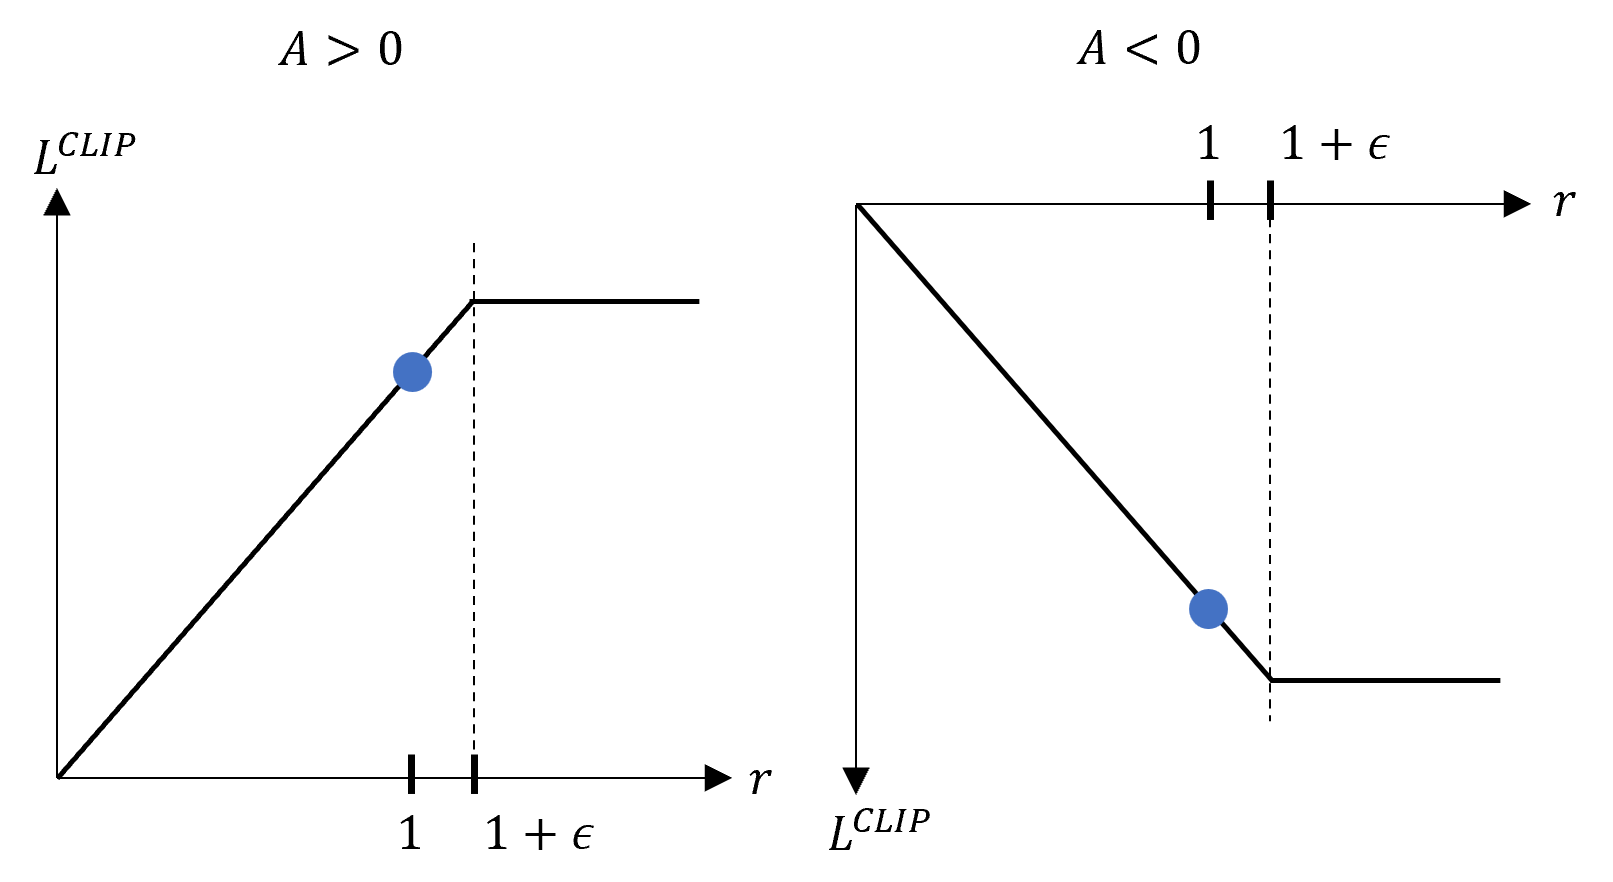
\includegraphics[width=0.6\linewidth]{fig/clip_function.png}
    \caption{Illustration of the clip function, where the probability ratio $r$ is clipped at $1-\epsilon$ or $1+\epsilon$ depending on the polarity of the advantage}
    \label{fig: clip function}
\end{figure}

The core philosophy of the PPO algorithm is to mitigate the challenges caused by large policy updates in the PG algorithm, which can it difficult for step sizes determination and low data efficiency. By adopting a clipping mechanism to avoid imposing hard constraint completely, the PPO is proven to be very effective in dealing with a wide range of challenging tasks, while being simple to implement and tune.

The architecture for the TTWR autonomous parking mechanism is depicted in Figure \ref{fig: TTWR training process}. This system is bifurcated into two primary components: a profound reinforcement learning module and a simulation framework. Specifically, the profound reinforcement learning module utilizes an LSTM-PPO technique to train the agent for mastering autonomous parking and evading obstacles, all while engaging with the entities within the parking milieu. The simulation framework encompasses the kinematic model of TTWR, static vehicular obstructions, parking spaces, and sonar-driven distance sensing, all realized in Matlab to engage with the training agent.

\begin{figure}[h]
    \centering
    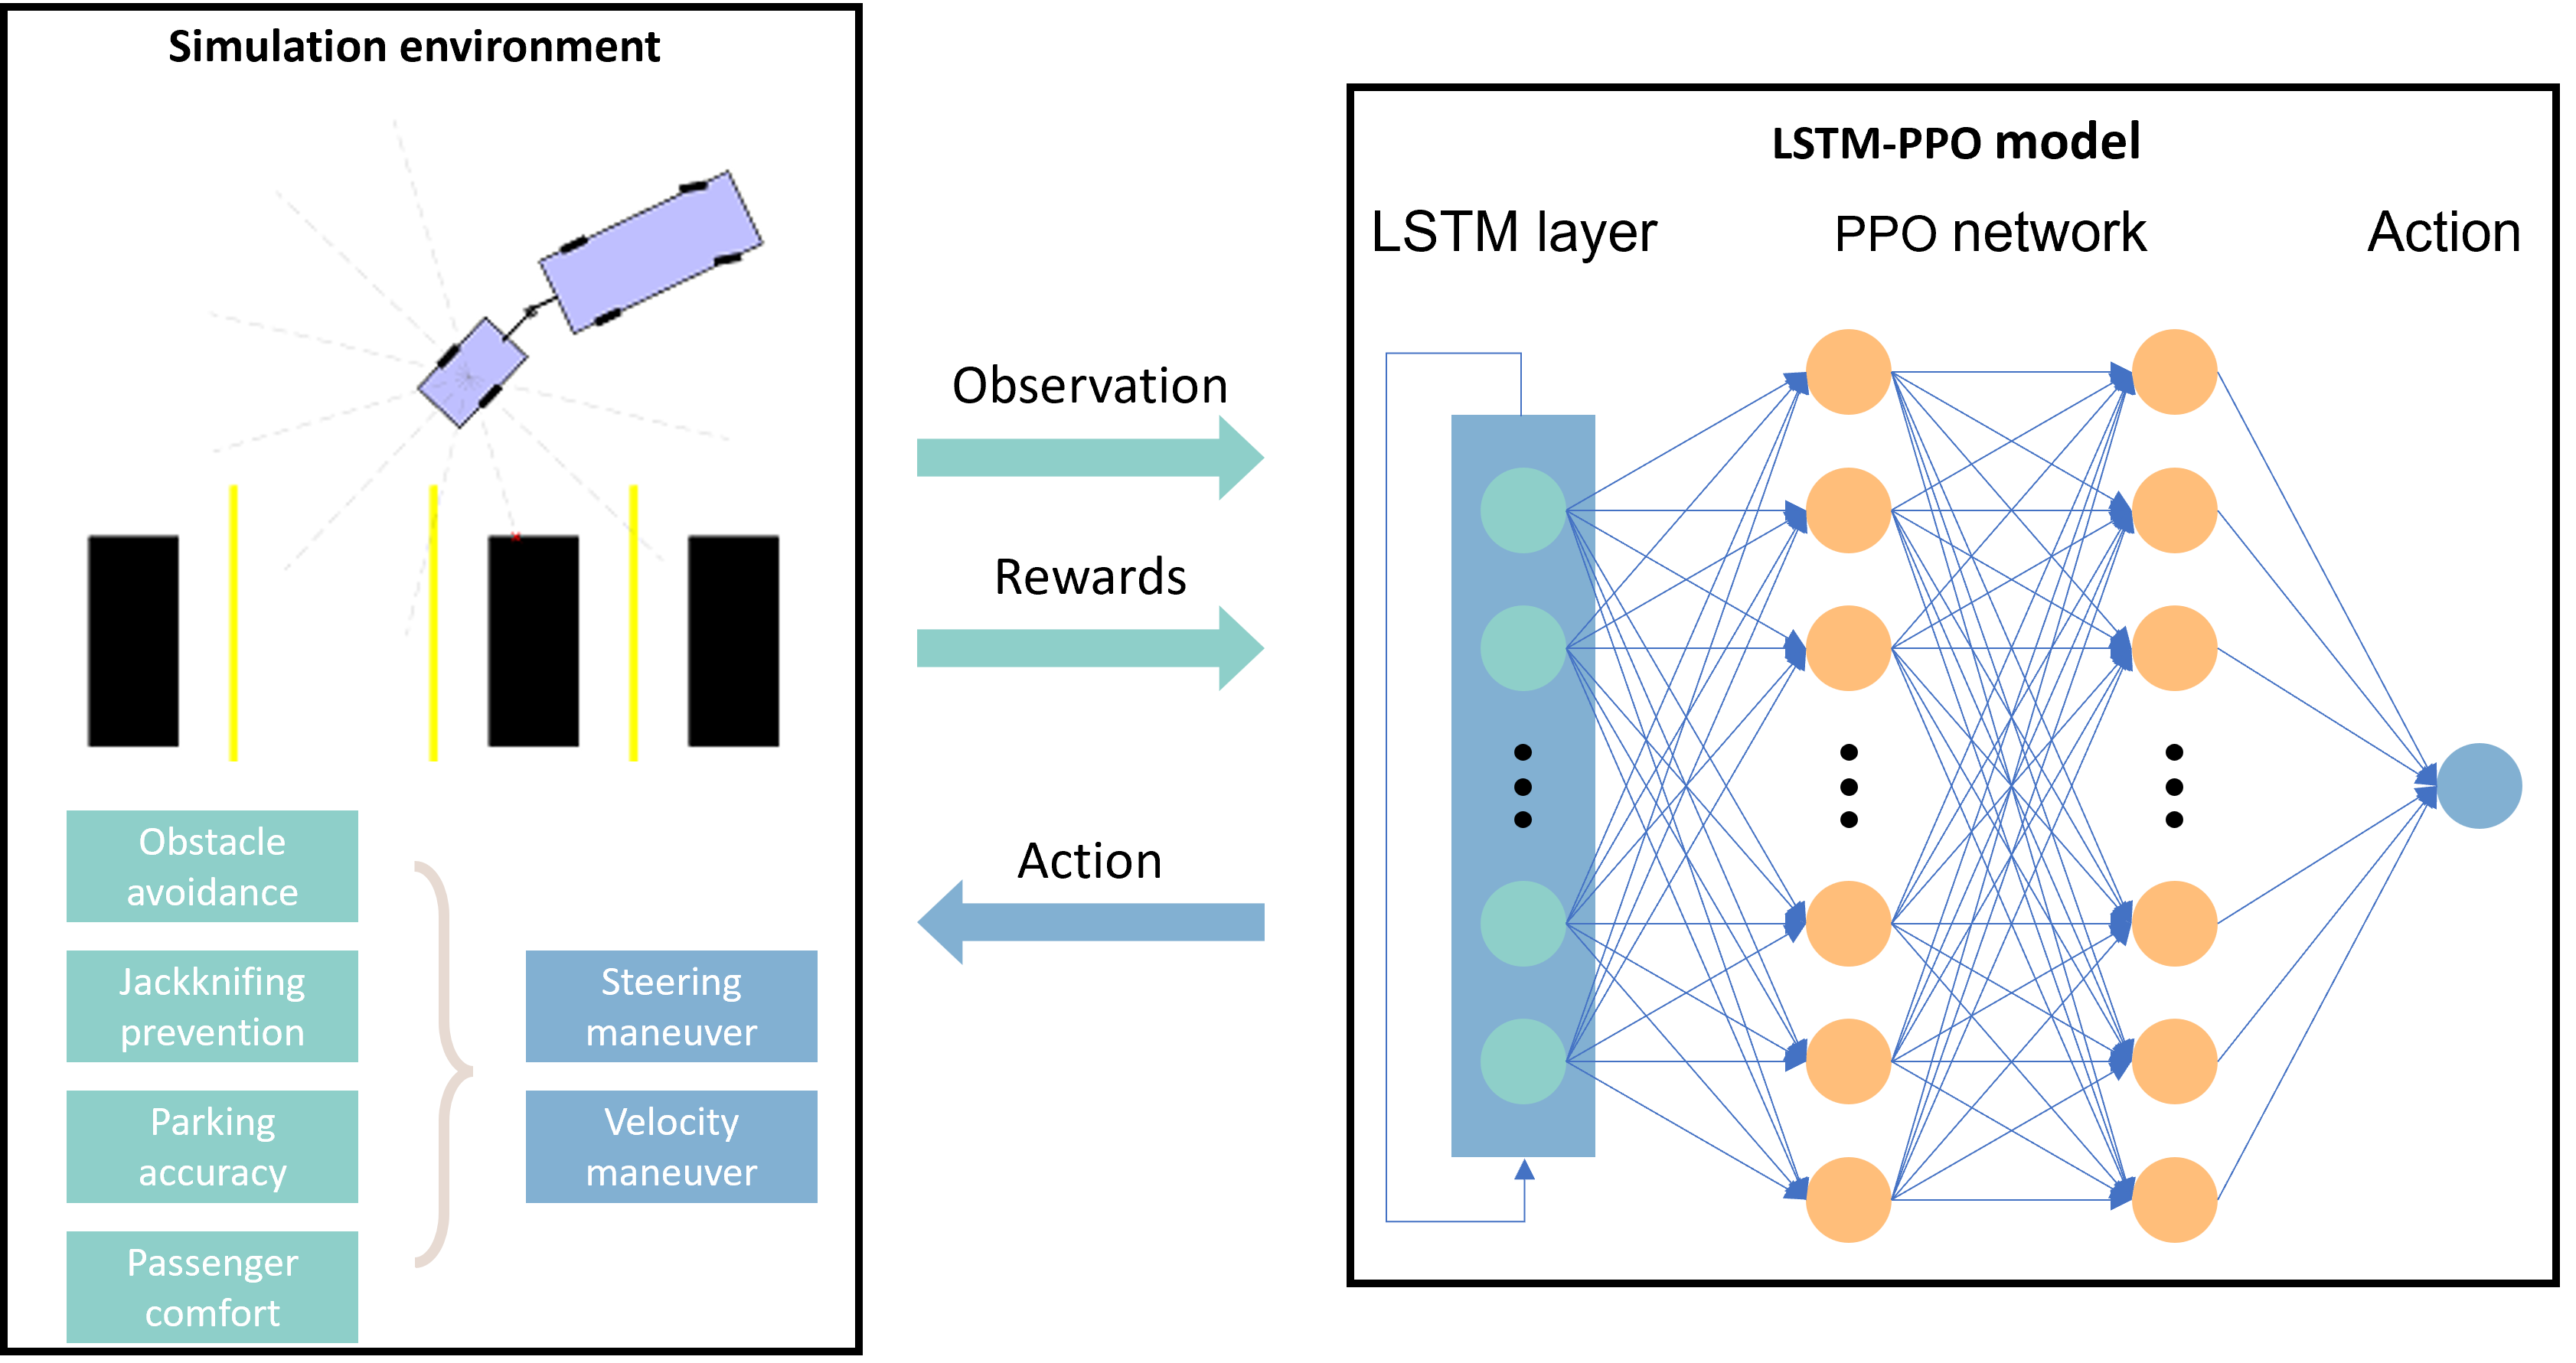
\includegraphics[width=0.9\linewidth]{fig/ppo/system_architecture.png}
    \caption{TTWR autonomous parking system layout}
    \label{fig: TTWR training process}
\end{figure}

The TTWR mechanism evaluates the parking target coordinates, TTWR system configurations, and the perceived obstacle data to execute the autonomous parking operation. To address the dimensionality challenges stemming from intricate observation data, the technique discretizes the obstacle perception data around the agent, sampling points within a predefined threshold. This allows for a more streamlined observation vector, represented as:

\begin{equation}
S_t = \left[\begin{array}{ccc}
S_\text{TTWR}, S_\text{sonar}, S_\text{goal}
\end{array}\right]^T
\label{eq: observation}
\end{equation}

Here, $S_\text{TTWR} = \left[\begin{array}{ccc} x_1, y_1, \theta_1, x_2, y_2, \theta_2, \phi\end{array}\right]^T$ represents the TTWR state configurations as defined by the kinematic model. The parking objective, $S_\text{goal} = \left[\begin{array}{ccc} x_\text{goal}, y_\text{goal}, \theta_\text{goal}\end{array}\right]^T$, signifies the desired parking location for the TTWR, determined by user input.

Furthermore, $S_\text{sonar}$ is the data from sonar instruments affixed to the trailer. Instead of a full $360^{\circ}$ environmental scan, the sonar provides distance measurements within its field of view. These readings can be transformed from polar to Cartesian coordinates to depict obstructions around the trailer. Specifically, the sonar readings, $S_\text{sonar}$, can be articulated as:

\begin{equation}
S_\text{sonar}=\left[\begin{array}{cccc}
dist_{1} & dist_{2} & \cdots & dist_{n}
\end{array}\right]
\label{eq: sonar observation}
\end{equation}

To enhance the driving experience and ensure fluid vehicle control, this study introduces an action module that represents the primary vehicle's steering input for lateral management. The steering controller prompts the agent to select the optimal action value from a continuous action domain, produced by the LSTM-PPO algorithm, and is defined within the range of $[-\delta_{max}, \delta_{max}]$, where $\delta_{max}$ is the utmost steering angle based on the primary vehicle's specifications.

The reward function acts as the feedback conduit for the controller, associating the current state and action of the TTWR to a scalar metric that evaluates potential maneuvers. Specifically, the reward function is crafted to guide the controller in learning how to adeptly park the trailer, emphasizing collision prevention and ensuring a seamless user experience.

\begin{itemize}
  \item Distance metric $R_{\text{dist}}$: Assesses the gap between the trailer's position and the parking space;
  \item Parking metric $R_{\text{parking}}$: Rewards the trailer when parked within the slot, adhering to specified tolerances;
  \item Steering constraint $R_{\delta}$: Penalizes excessive steering maneuvers to bolster passenger comfort;
  \item Collision constraint $R_{\text{collision}}$: Penalizes when the TTWR system nears surrounding entities;
  \item Jackknife avoidance $R_{\phi}$: Assesses the risk when nearing a jackknifing scenario.
\end{itemize}

As illustrated in Figure \ref{fig: TTWR training process}, the distance metric $R_{d}$ is provided in every iteration to motivate the TTWR to gravitate towards the designated parking slot. This is defined as:

\begin{equation}
R_{\text{dist}}(s_t, a_t, s_{t+1}) = e^{-(s_t^2 + s_\text{goal}^2)}
\label{eq: distance reward}\end{equation}

The parking metric $R_{\text{park}}$ is allocated when the trailer adeptly parks itself within the parking slot, adhering to state tolerance $s_{\epsilon}$. The additional accuracy metric is gauged by the distance between the concluding state $s_{\text{final}}$ and goal state $s_{\text{goal}}$:

\begin{equation}
R_{\text{parking}}
=
\left\{\begin{array}{l}
c- \frac{ \lVert s_\text{final}-s_\text{goal} \rVert }{s_{\epsilon}}, \text { if } \lVert s_\text{final}-s_\text{goal} \rVert \leq s_{\epsilon}\\
0, \text { otherwise }
\end{array}\right.
\label{eq: parking reward}\end{equation}

Additionally, the collision penalty $R_c$ is applied when the distance between TTWR and surrounding obstructions falls within a threshold, ending the ongoing episode to indicate a collision. The jackknife penalty $R_{\phi}$ is proportional to the $\phi$ value, promoting minor maneuvers, and the steering penalty is proportional to the steering value to deter large $\delta$ inputs.

The comprehensive parking reward, encompassing all four components, is expressed in Eqn. \ref{eq: total rewards}:

\begin{equation}
R=R_{\text{collision }} + R_{\text{parking}} + R_{\text{collision}} + R_{\delta} + R_{\phi}
\label{eq: total rewards}\end{equation}

Figure \ref{fig:perpendicular parking} showcases the trajectory of perpendicular parking simulation outcomes, validating that the proposed LSTM-PPO controller can adeptly modify the TTWR system's inputs, including host velocity and steering angle, to approach the chosen parking spot during the perpendicular parking task. The starting positions are initialized with a certain degree of noise, and the goal position is determined by user input. The dotted trajectory represents the trailer's path, with two faded TTWRs indicating its initial and concluding positions. In Figure \ref{fig:parking_system_states}, the trailer's states during the parking task are displayed in the global coordinate system, aligning with the chosen parking spot's coordinates and orientation.

\begin{figure}
     \centering
     \begin{subfigure}[b]{0.4\textwidth}
         \centering
         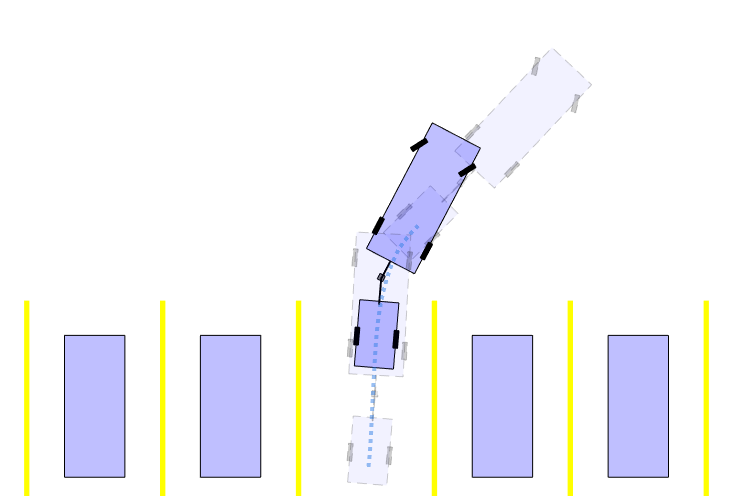
\includegraphics[width=\textwidth]{fig/ppo/parkingIllustration.png}
         \caption{Perpendicular parking simulation}
         \label{fig:parking_trajectory_1}
     \end{subfigure}
     \hfill
     \begin{subfigure}[b]{0.4\textwidth}
         \centering
         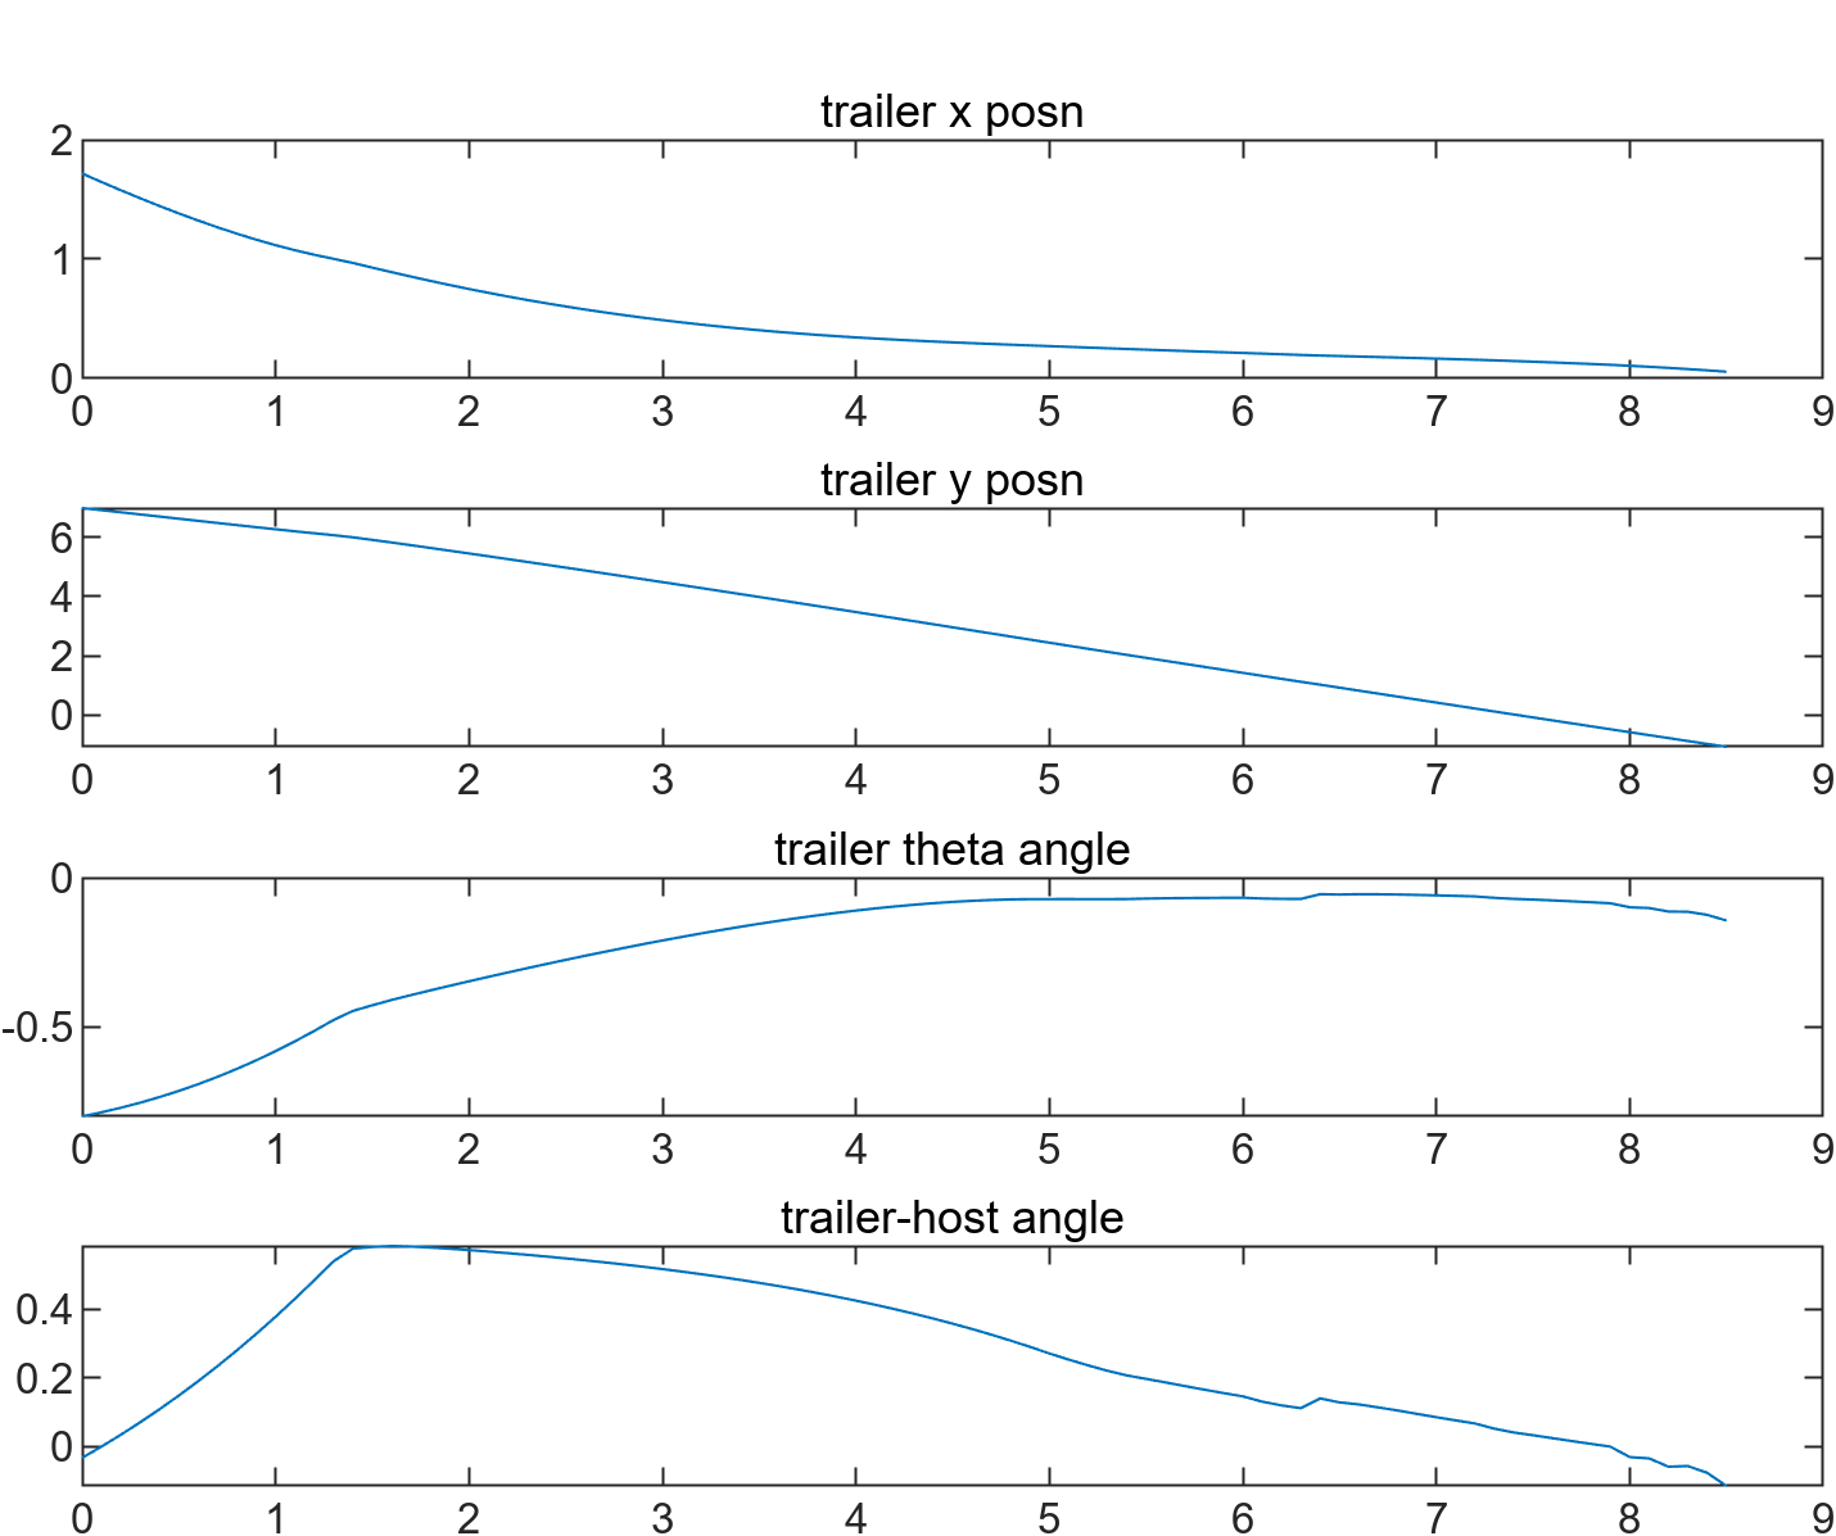
\includegraphics[width=\textwidth]{fig/ppo/parking_system_states.png}
         \caption{Perpendicular parking system states}
         \label{fig:parking_system_states}
     \end{subfigure}
        \caption{TTWR perpendicular parking}
        \label{fig:perpendicular parking}
\end{figure}

In Figure \ref{fig:oblique parking}, the TTWR trajectory during a $45^{\circ}$ oblique parking simulation is depicted. Similarly, the starting positions are initialized with a certain degree of noise, and the proposed methods successfully parked the TTWR system, ensuring jackknife prevention and obstacle evasion.

\begin{figure}
     \centering
     \begin{subfigure}[b]{0.4\textwidth}
         \centering
            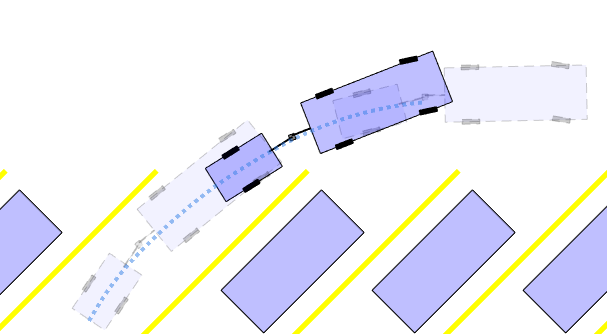
\includegraphics[width=\textwidth]{fig/ppo/parkingIllustration_oblique.png}
            \caption{Oblique parking system states}
            \label{fig:parking_trajectory_oblique_illustration}
     \end{subfigure}
     \hfill
     \begin{subfigure}[b]{0.4\textwidth}
         \centering
            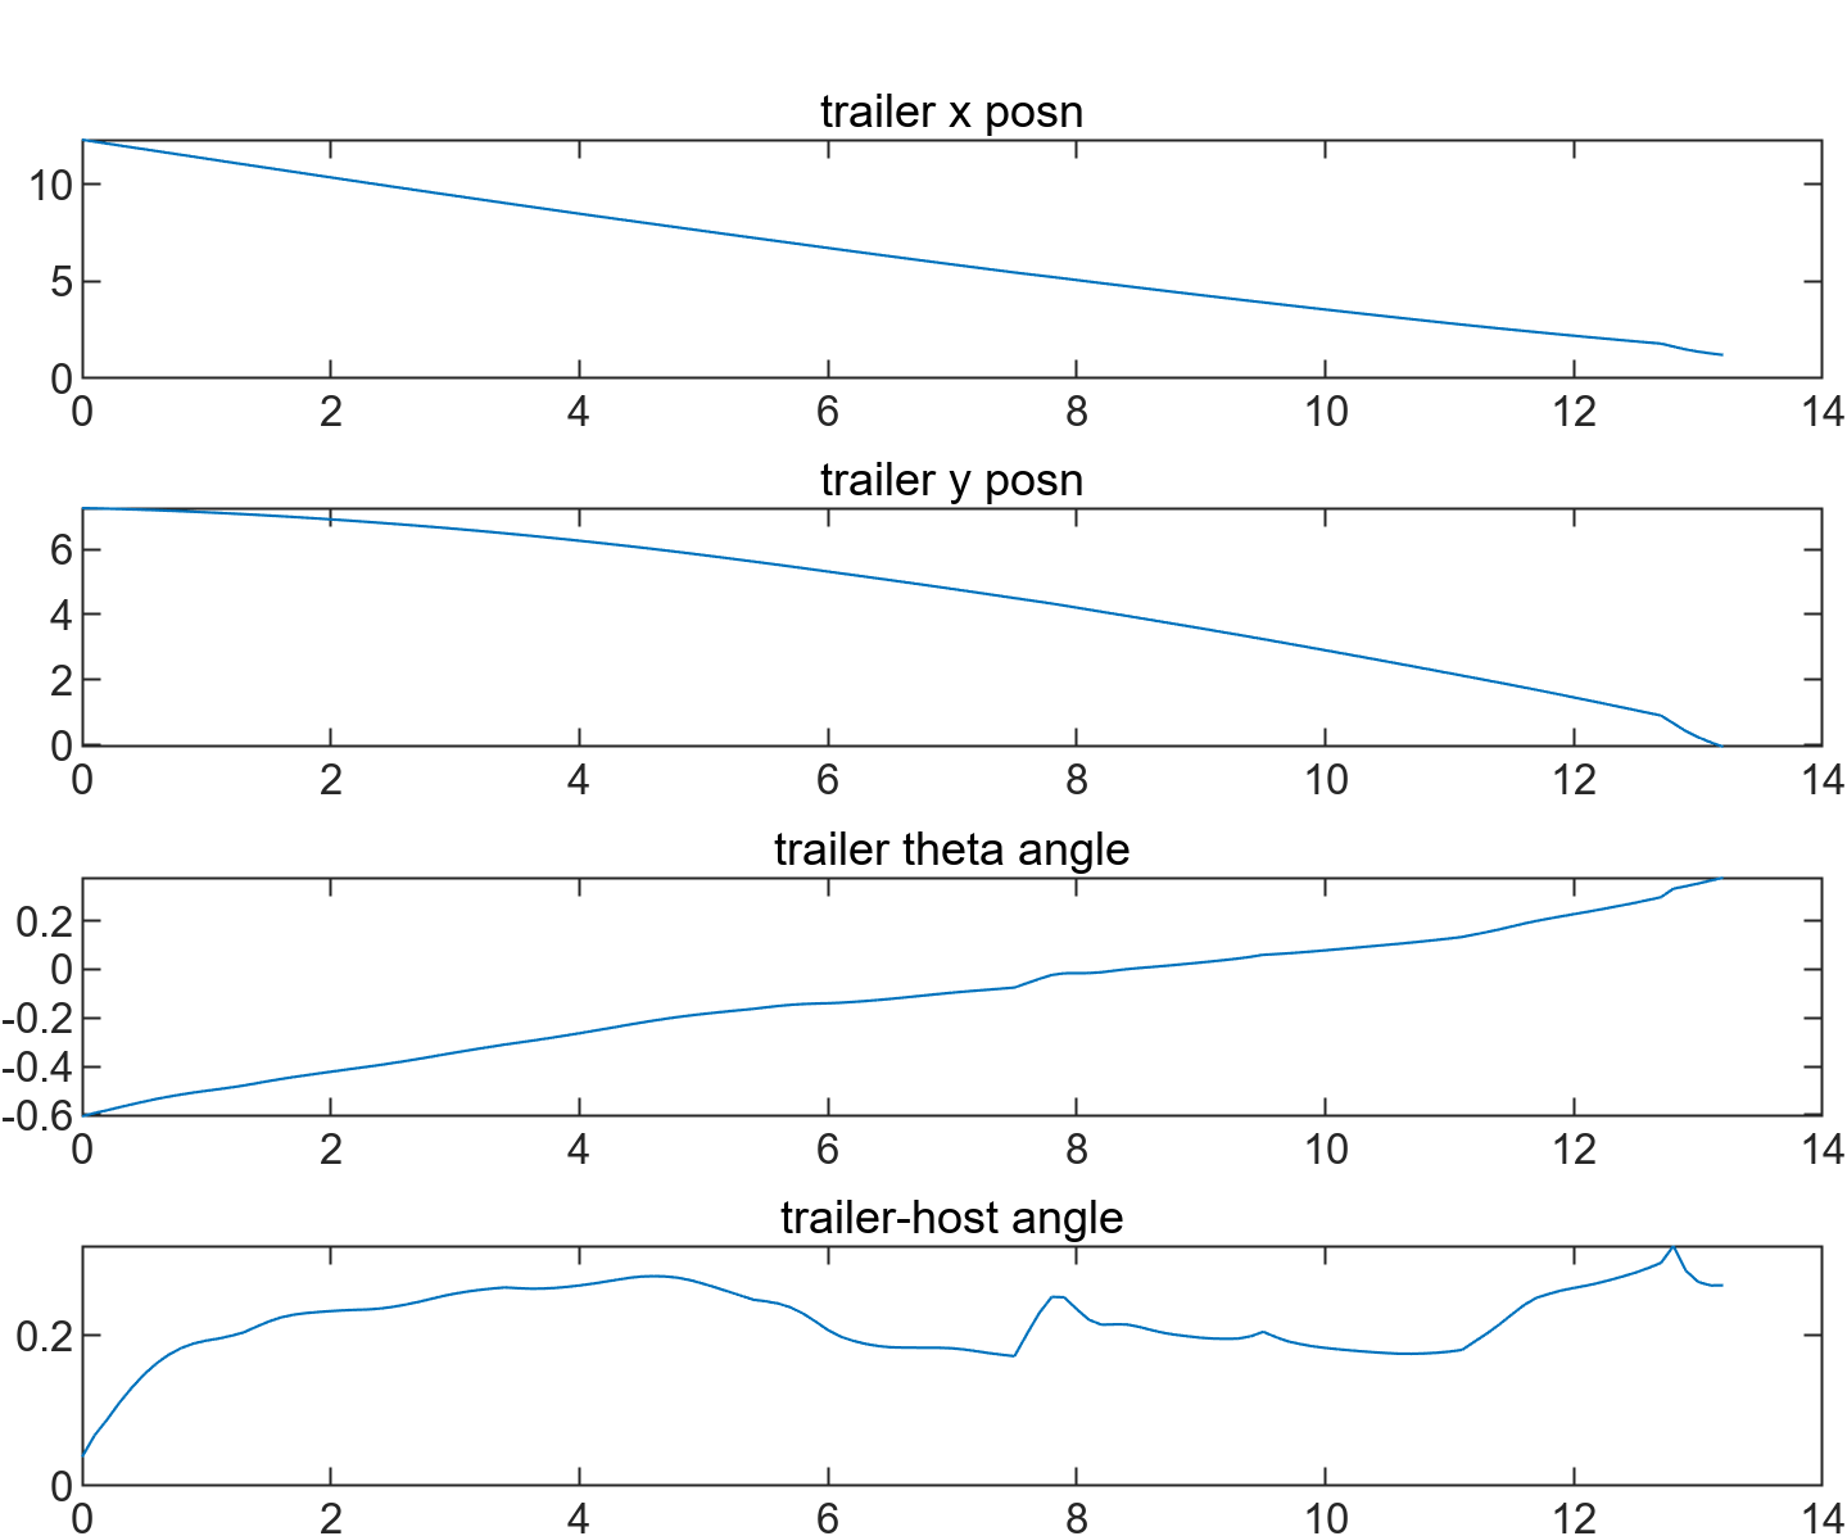
\includegraphics[width=\textwidth]{fig/ppo/parking_system_states_oblique.png}
            \caption{Oblique parking system states}
            \label{fig:parking_system_states_oblique}
     \end{subfigure}
        \caption{TTWR oblique parking}
        \label{fig:oblique parking}
\end{figure}


\section{Trajectory state model-based reinforcement learning for TTWR reverse parking}
\label{section: Trajectory state model-based reinforcement learning for TTWR reverse parking}

* this section is from the submitted second paper which does not provide citation for now.

By employing the trajectory state prediction model as the foundation model to interact with the Proximal Policy Optimization framework, we enable reversible access to the Markov Decision Process dynamics and help the PPO to better estimate vehicle dynamics used for controller. A numerical simulation is conducted to demonstrate the trajectory following accuracy of the proposed methodology compared with popular industry control methods such as linear–quadratic regulator. Our results indicate that the proposed hybrid trajectory model based approach not only reduces the need for extensive data collection but also achieves similar control accuracy, suggesting a promising direction for future research in autonomous vehicle control, emphasizing the need for efficient, adaptable, and robust learning algorithms.

\begin{figure}[h]
    \centering
    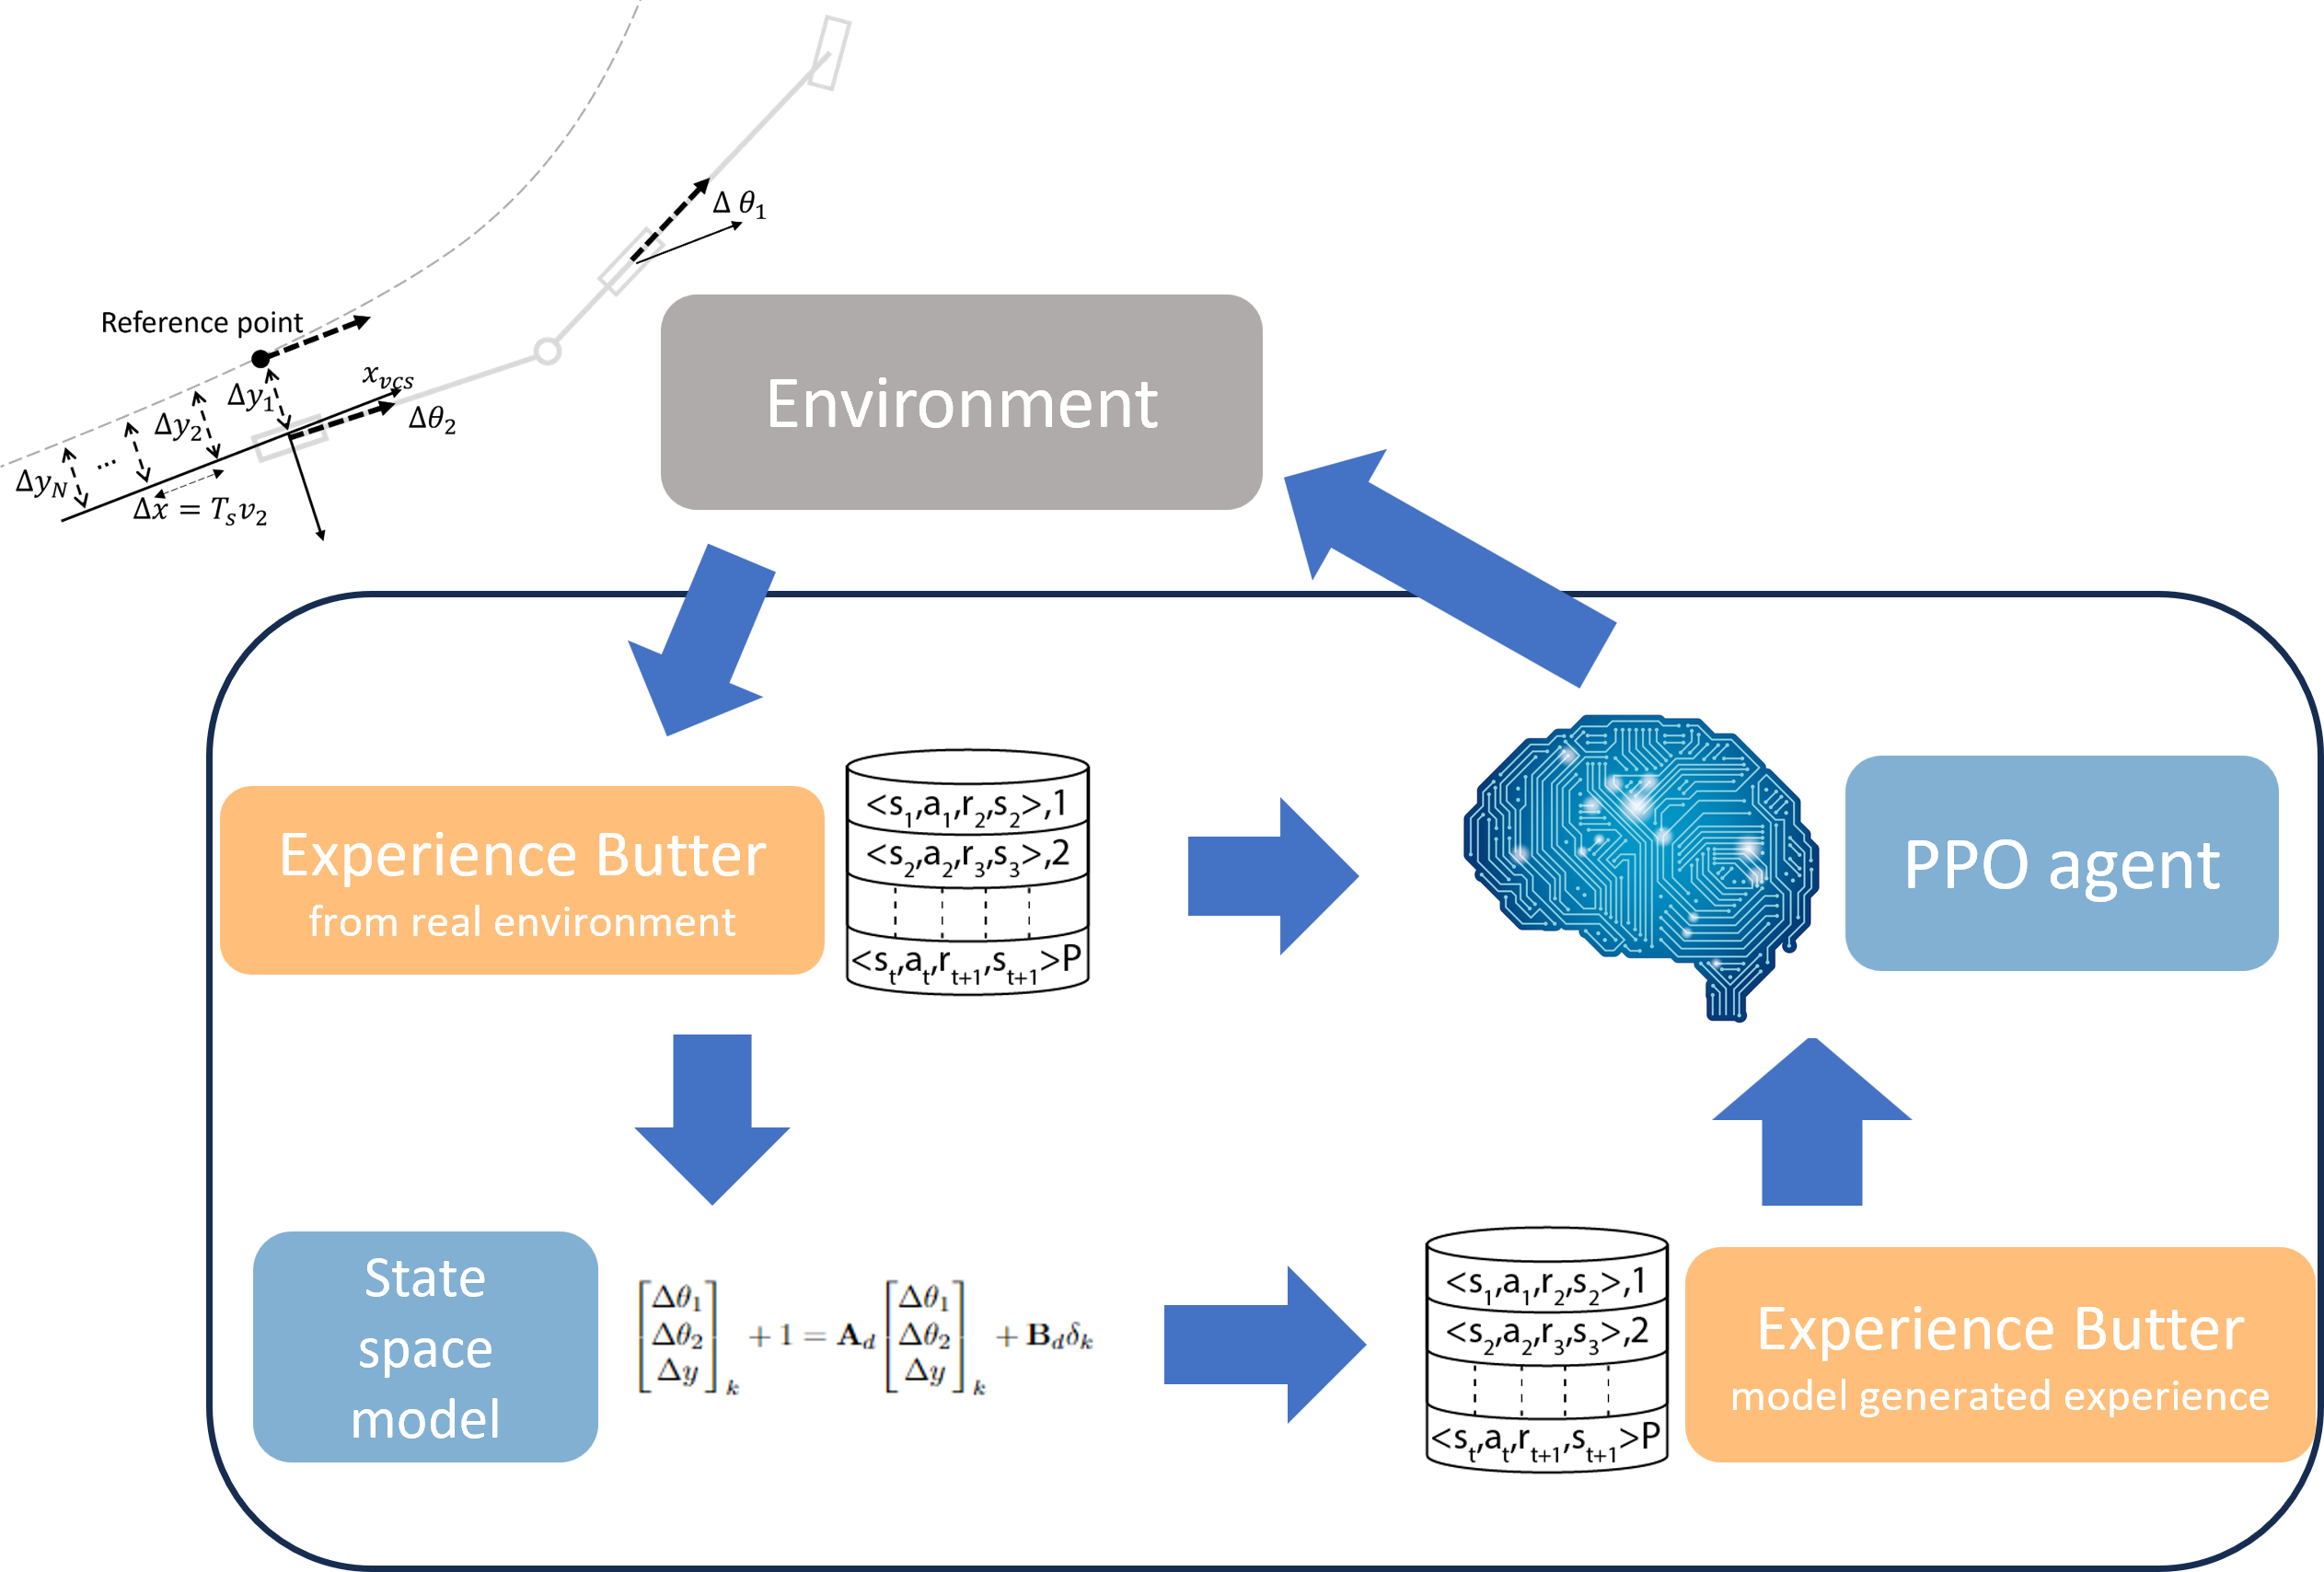
\includegraphics[width=0.8\linewidth]{fig/known mbrl schema.png}
    \caption{The MBRl structure with Dubins trajectory model generator}
    \label{fig: The MBRl structure with Dubins trajectory model generator}
\end{figure}

While model-free deep reinforcement learning has achieved remarkable successes across various domains, its application remains limited by substantial sample inefficiency and a lack of interpretability. Model-based reinforcement learning algorithms are generally regarded as being more efficient, the model-based policy search methods tackle the challenge of sample inefficiency by utilizing observed trajectories to construct a predictive model of the robot's dynamics and interactions with its surroundings \cite{schulman2015trust}. However, previous works have relied on straightforward function approximators \cite{lioutikov2014sample} or Bayesian models \cite{deisenroth2011pilco} to maintain sample efficiency and prevent overfitting. The application of these methods to diverse and intricate high-dimensional tasks is challenging. Efforts to address these issues have included the use of large-scale neural networks to capture the intricate dynamics typical of deep reinforcement learning benchmarks. However, these models often require extended training periods and struggle with transferability and interpretability \cite{nagabandi2018neural}, which confines the application scope of these models to tasks with relatively static scenarios and assignments.

By integrating the Dubin path planning with preview control, we build the system dynamics model to represent the environment interaction, where the preview distance control is also applied. In Figure \ref{fig:Vehicle kinematics model with reference}, the first $N$ preview reference points and the deviation value are plotted within the trailer VCS, and the reference error value for each preview reference sample is computed and denoted by $(\theta_{1_k}, \theta_{2_k}, y_k)$, $\Delta x$ is the sampling interval and $T_s$ is the simulation step time. Therefor, the $N$ preview sample points can be computed by:

\begin{equation} 
 {\begin{bmatrix}
    \Delta \theta_1 \\ \Delta \theta_2 \\ \Delta y
\end{bmatrix}}_k+1 = \mathbf{A}_d {\begin{bmatrix}
    \Delta \theta_1 \\ \Delta \theta_2 \\ \Delta y
\end{bmatrix}}_k + \mathbf{B}_d \delta_k
\end{equation}
where
\begin{flalign*}
A_r&=\left[\begin{array}{ccccc}
0 & 1 & 0 & \cdots & 0 \\
0 & 0 & 1 & \cdots & 0 \\
\vdots & \vdots & \vdots & \ddots & \vdots \\
0 & 0 & 0 & \cdots & 1 \\
0 & 0 & 0 & \cdots & 0
\end{array}\right]_{(N \times N)} \quad 
\end{flalign*}
and
\begin{flalign*}
B_r&=\left[\begin{array}{c}
0 \\
0 \\
0 \\
\vdots \\
1
\end{array}\right]_{(N \times 1)}
\end{flalign*}
\begin{figure}[h]
\centering
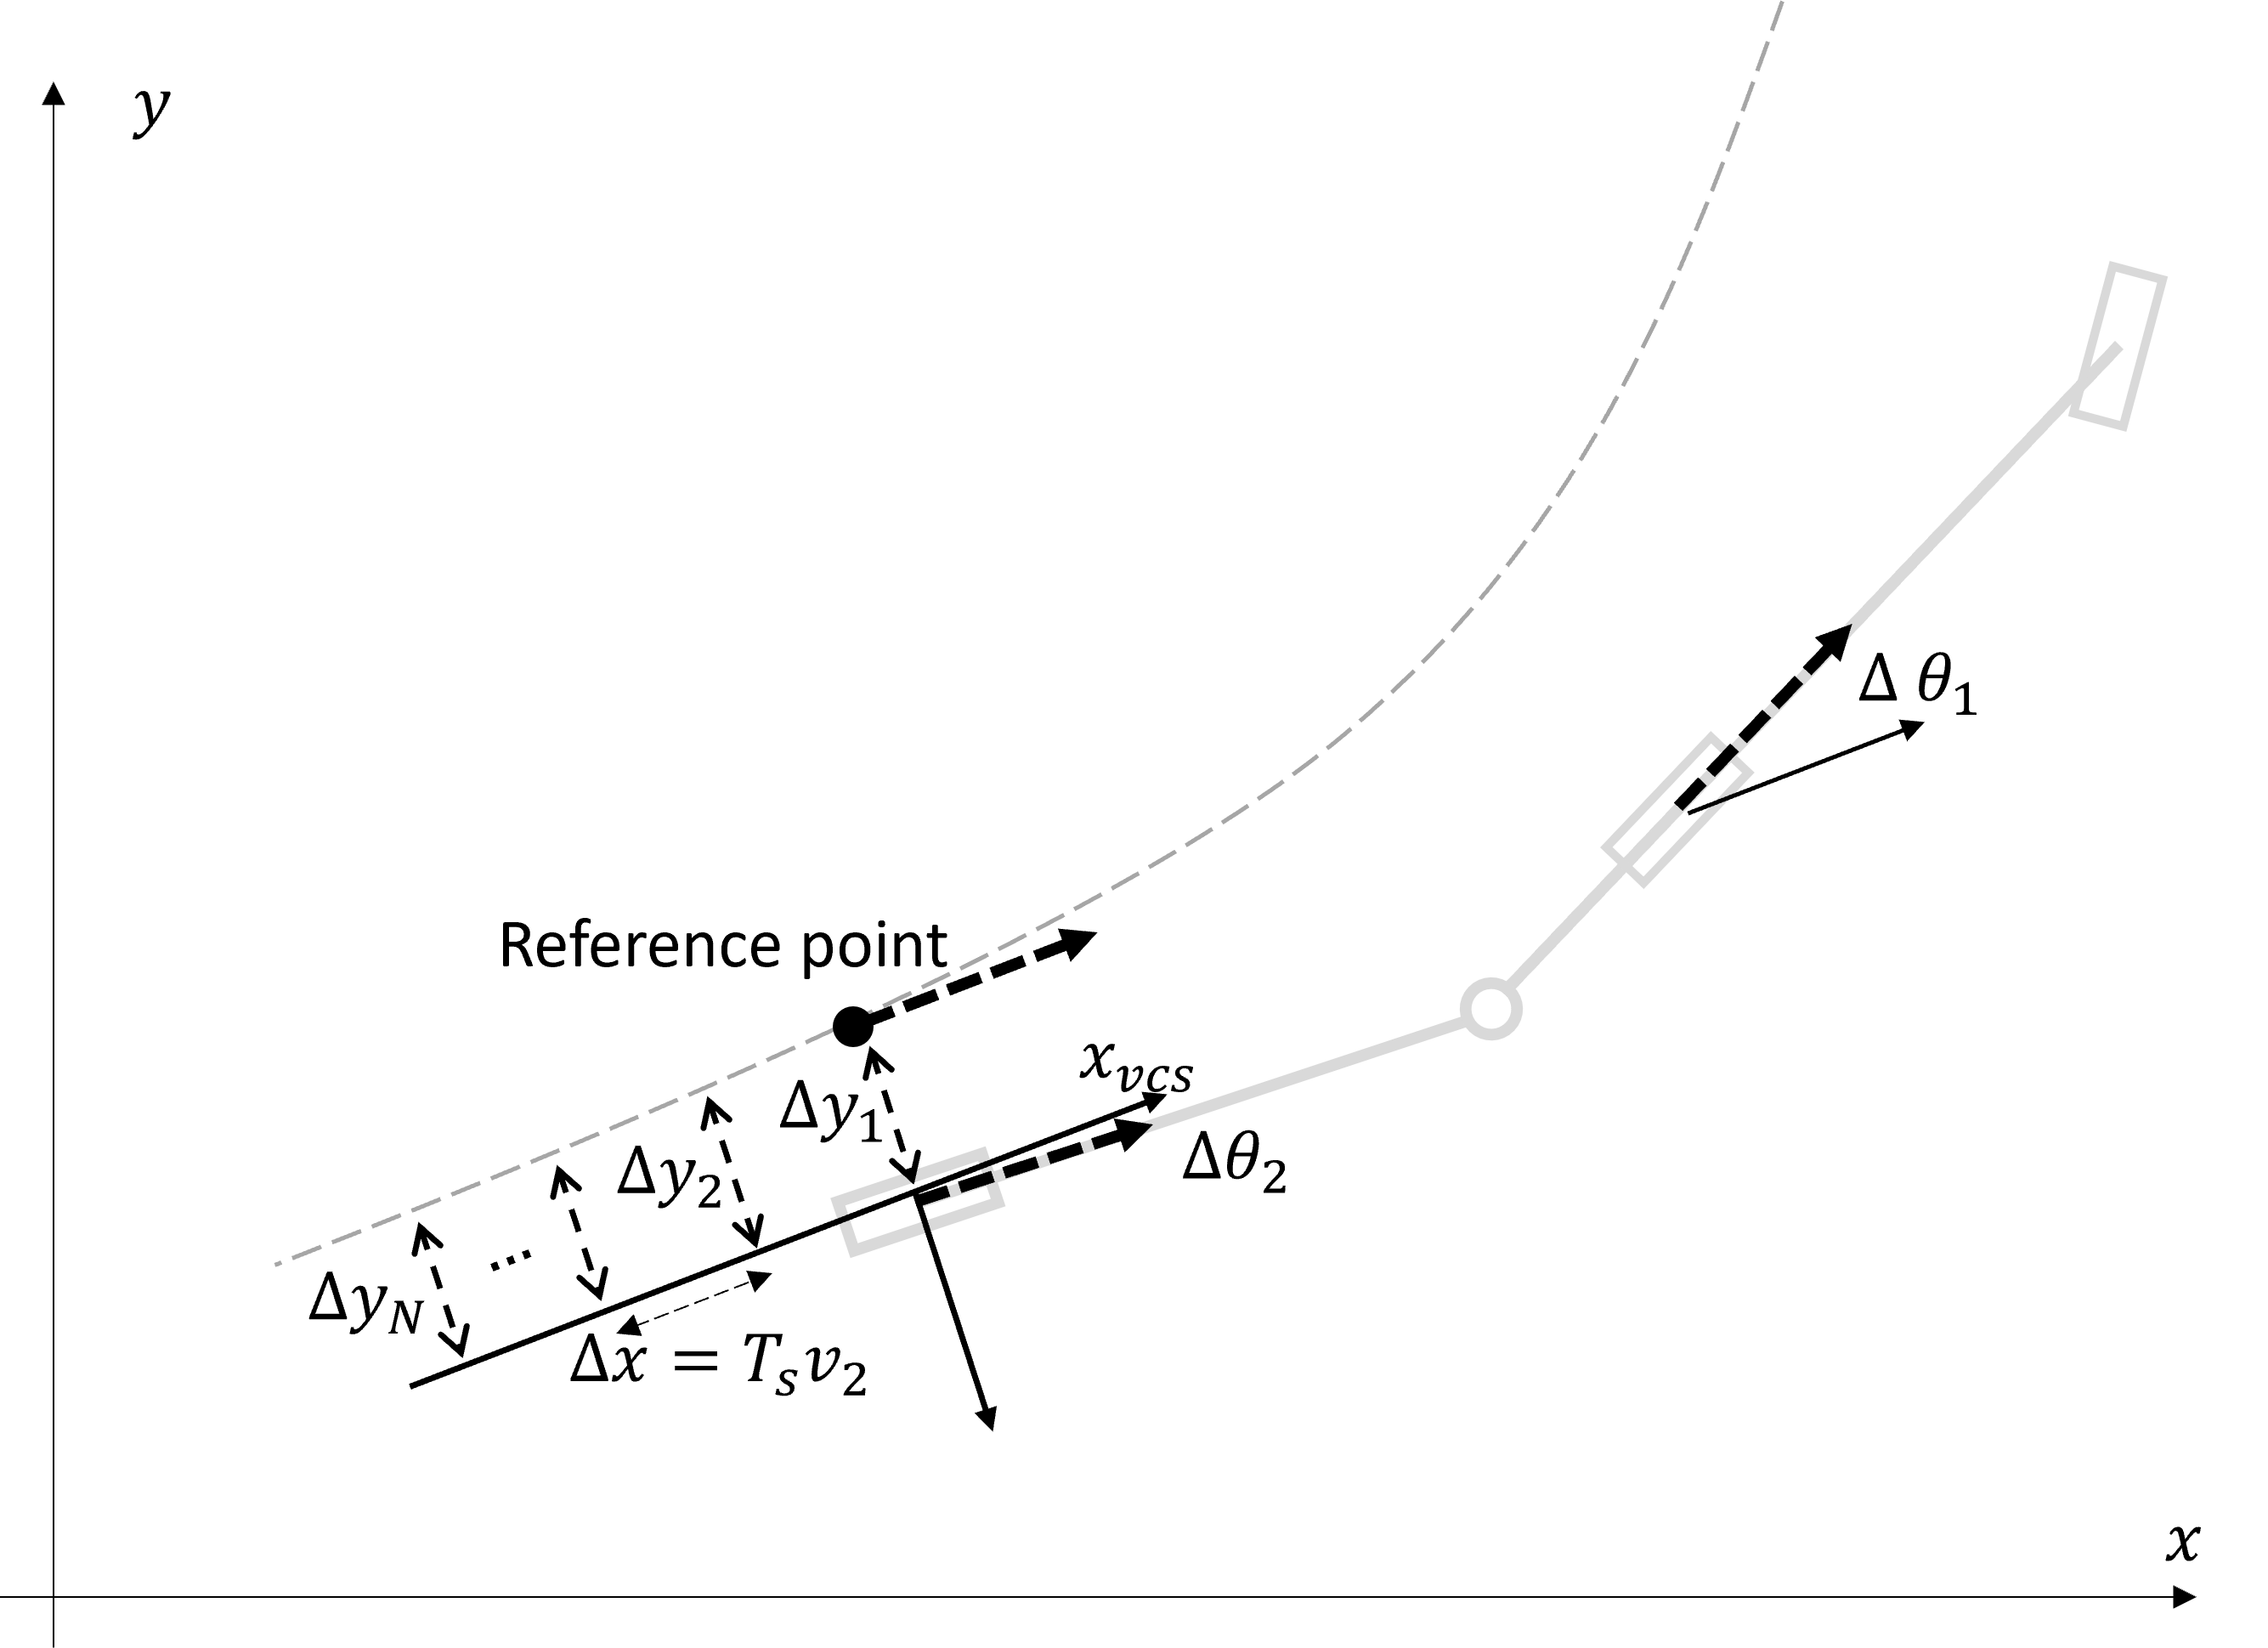
\includegraphics[width=0.8\linewidth]{fig/knownMBRL/lateral distance error.png}
\caption{Vehicle kinematics model with reference}
\label{fig:Vehicle kinematics model with reference}
\end{figure}

We evaluate the effectiveness of the proposed learning strategy using the benchmark platform across various vehicle setups for trajectory tracking tasks. The initialization of the trajectory planning and motion prediction models were based on the kinematic state space model of the vehicles which requires a single calibration for each agent. Subsequently, these models networks can be transferred and re-trained during operation to manage distinct tasks for changing vehicle configurations. The adaptability of our method was evident as it successfully handled new challenges during testing, such as managing trailers with increased overhang length which introduced more intricate dynamics.


\begin{figure}[htbp]
\centerline{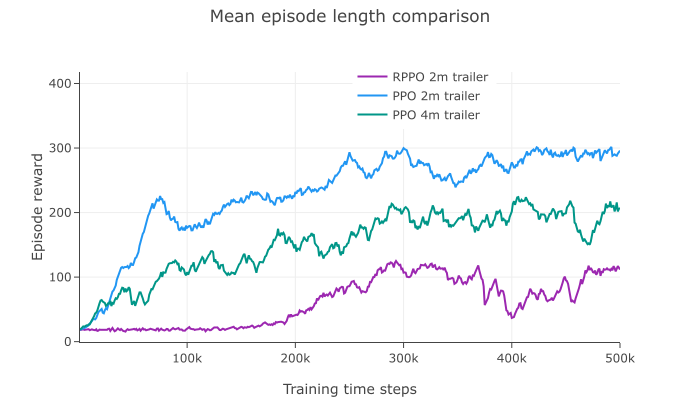
\includegraphics[width=0.8\linewidth]{fig/knownMBRL/Mean episode length.png}}
\caption{Mean episode length comparison between RPPO training on 2 meters trailer, PPO training on both 2 meters and 4 meters trailer}
\label{fig:Mean episode length}
\end{figure}

Figure \ref{fig:Mean episode length} compares the mean episode lengths for PPO-trained agents with 2-meter and 4-meter trailers as well as an RPPO-trained agent trained with 2-meter trailer. The PPO agent trained with a shorter trailer shows better performance, achieving efficient parking after 250,000 training steps. In contrast, the longer trailer brings more complexity for reverse driving maneuvering, which leads to a slower training, although it achieves similar parking success rate and rewards in \ref{fig:Mean episodic training reward}. However, the success rate of RPPO algorithm is under $50\%$ and the training takes more steps, possibly due to vanishing gradients and the intricate nature of the task's delayed rewards.

\begin{figure}[htbp]
\centerline{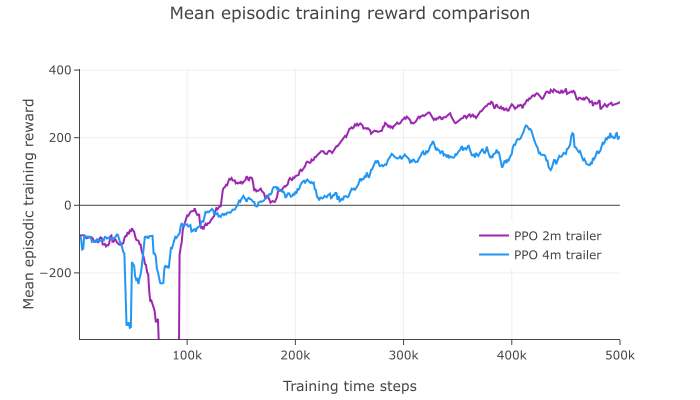
\includegraphics[width=0.8\linewidth]{fig/knownMBRL/Mean episodic training reward.png}}
\caption{Mean episode training reward comparison between PPO training on both 2 meters and 4 meters trailer}
\label{fig:Mean episodic training reward}
\end{figure}

Figure \ref{fig:Mean episodic training reward} shows that the PPO with a 2-meters trailer is able to achieving stable rewards by 250,000 steps. The training of 4m trailer's catches up by 300k steps, reflecting the added complexity in controlling longer trailers and the consequent need for extended training to refine the parking maneuvers.

\begin{figure}[htbp]
\centerline{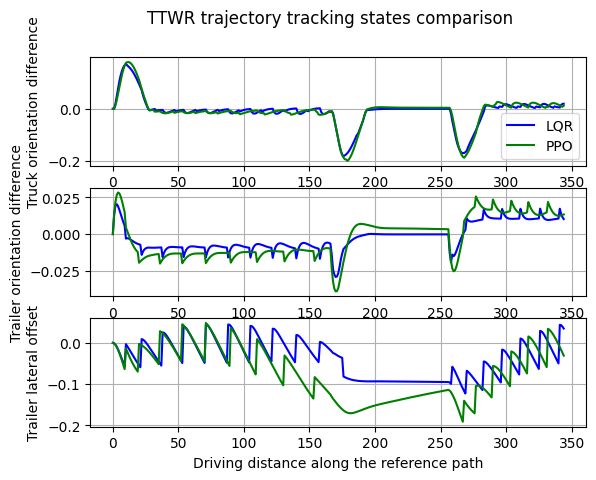
\includegraphics[width=0.8\linewidth]{fig/knownMBRL/comparison of lqr ppo.png}}
\caption{The comparison of LQR controller and proposed algorithm controlling normal 2m trailer v.s. reference trajectory orientation error, trailer orientation error, and trailer lateral offset error}
\label{fig: parking error comparison}
\end{figure}

\begin{figure}[htbp]
    \centerline{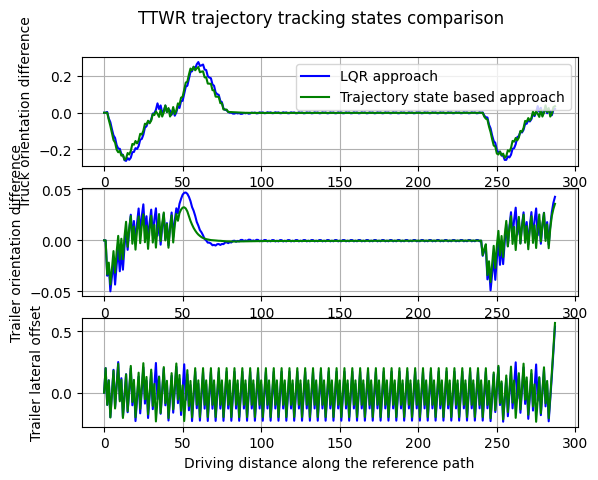
\includegraphics[width=0.8\linewidth]{fig/knownMBRL/comparison of lqr ppo extended vehicle.png}}
    \caption{The comparison of LQR controller and proposed algorithm controlling extended trailer v.s. reference trajectory orientation error, trailer orientation error, and trailer lateral offset error}
    \label{fig: parking error comparison of extended trailer}
\end{figure}

Figure \ref{fig: parking error comparison} compares the LQR controller with the proposed algorithm regarding truck orientation error, trailer orientation error, and lateral offset error. For a 2-meter trailer which is popular in North America market which handles most moving tasks, the performance of both systems is closely matched, with the lateral offset consistently maintained below 0.2 meters. The result shows the proposed algorithm's high tracking accuracy and suggests its potential effectiveness in practical scenarios.

Figure \ref{fig: parking error comparison of extended trailer} presents a comparative analysis of the LQR controller and the proposed algorithm, applied to a 5-meter extended trailer designed for heavy-duty tasks. Both controllers successfully follow the given trajectory; however, the proposed algorithm demonstrates slightly better performance in orientation tracking with smaller errors. This indicates enhanced adaptability of the proposed algorithm in contrast to the LQR controller, which relies on fixed feedback gains.